% !TeX root = main.tex
\cleardoublepage
\fancyfoot[L]{\small \RomanNumeralCaps{3}}

\section{Physical foundations of optical spectroscopy; electron, oscillatory and rotational excitations of particles and the corresponding ranges of the spectrum of electromagnetic radiation}
\label{sec:spectroscopy}
 
    Optical spectroscopy is an analytical technique which studies the interaction of electromagnetic radiation with matter. By analysing the absorption, emission or scattering of light by atoms and molecules, one obtains information about their electronic, vibrational and rotational structure.
 
    A molecule can store energy in three ways, and they differ greatly in the amount of energy involved. In decreasing order of energy these are \emph{electronic}, \emph{vibrational} and \emph{rotational} excitations, each about one to two orders of magnitude below the one above it. The three can be counted separately because the electrons are thousands of times lighter than the nuclei and so follow any nuclear motion instantly---the \emph{Born--Oppenheimer approximation}---which lets the state of a molecule be labelled by one quantum number from each of the three, with the total energy their sum.\todoans{These do not compete with the atomic $n$, $l$, $m$ scheme. Born--Oppenheimer factorises the wave function, $\psi \simeq \psi_{\text{el}}\psi_{\text{vib}}\psi_{\text{rot}}$. The electronic factor is the molecular counterpart of the atomic orbitals of \cref{sec:atom-molecule}, whereas $v$ and $J$ describe the \emph{nuclei}---how the bonds stretch and how the whole frame turns---and have no atomic analogue.}
 
    In molecules all three are present at once, so a single electronic transition carries a whole comb of vibrational and rotational sub-levels on top of it, and this is what turns what would be one atomic line into a broad structured band. A transition changing the vibrational and the rotational state together gives a \emph{vibrational--rotational} band, and that is what the infrared spectrum of a gas consists of.\todoans{Standard names if you want them: \emph{rovibrational} for a vibrational--rotational band, \emph{rovibronic} when the electronic state changes as well. \enquote{Rotational--rotational coupling} is not standard usage. \emph{Spin--orbit coupling} is a different matter entirely---atomic fine structure, defined in \cref{sec:atom-molecule}---and has no place in this section.}
 
    A transition is only seen if the light can couple to it, which for infrared absorption and emission means that the vibration or the rotation must change the electric dipole moment of the molecule. A molecule of two identical atoms such as N$_{2}$ therefore has no infrared spectrum at all. CO$_{2}$ has no permanent dipole moment either, but its bending and asymmetric-stretch vibrations create one while they last, which is enough, and H$_{2}$O is polar to begin with---this is the whole basis of the greenhouse effect. Even N$_{2}$ is not blind to light in general, since it still has electronic transitions in the ultraviolet and it appears in Raman scattering (\cref{sec:light-matter}), which asks only that the polarisability (\cref{eq:polarisability}) change rather than the dipole moment.
 
    \subsection{Electronic excitations}
 
        Electronic excitations are jumps of an electron between the bound energy levels of an atom or molecule (\cref{sec:atom-molecule}). When a photon of the right energy is absorbed, an electron moves from a lower to a higher level, which shows as a line or band in the absorption spectrum. These are the largest steps, a few electronvolts, which puts them in the visible and near-ultraviolet, roughly \qtyrange{200}{800}{\nano\metre}. Visible light itself runs from about \qtyrange{380}{750}{\nano\metre}, that is from about \qty{790}{\tera\hertz} down to \qty{400}{\tera\hertz}.
 
    \subsection{Vibrational excitations}
 
        Vibrational excitations are oscillations of the atoms within a molecule about their equilibrium positions, for example the stretching or bending of a bond. Any potential minimum is harmonic for small displacements, so the levels are those of a harmonic oscillator, $E_{v} = \left(v+\nicefrac{1}{2}\right)\hbar\omega$ with $v = 0,1,2,\dots$ (\cref{sec:quantisation}), and are therefore evenly spaced. The spacing is of order \qty{0.1}{\electronvolt}, which places them in the infrared, roughly \qtyrange{2.5}{25}{\micro\metre}.
 
    \subsection{Rotational excitations}
 
        Rotational excitations are changes in the rotation of the whole molecule about its centre of mass, so they change its angular momentum, which is quantised as in \cref{sec:angular-momentum}. The levels are $E_{J} = BJ(J+1)$ with $J = 0,1,2,\dots$, so unlike the vibrational ladder they are not evenly spaced but spread out as $J$ grows, and the constant $B$ is inversely proportional to the moment of inertia---heavier molecules have more closely spaced levels. These are the smallest steps of the three, of order a few \unit{\milli\electronvolt} down to much less, giving wavelengths from a fraction of a millimetre to a few centimetres: the far infrared and the microwave region. Rotational spectra are the sharpest of the three.\todoans{$J$ obeys the same algebra as the electronic $l$ of \cref{sec:angular-momentum}---the same $J(J+1)$ pattern, the same $2J+1$ orientations---but it belongs to the \emph{nuclear frame} rather than to the electrons. It is a separate factor in the wave function, which is why the two sets of quantum numbers coexist without clashing.}

\section{Phenomena accompanying the interaction of electromagnetic radiation with atoms and molecules; stimulated and spontaneous emission, absorption}
\label{sec:light-matter}

    An atom or molecule with discrete energy levels can exchange energy with light in three basic ways: it can absorb a photon, emit one spontaneously, or be triggered to emit one by a passing photon. All three are \emph{resonant}, meaning they occur only when the photon energy $hf$ matches the gap between two levels.

    Light whose energy matches no level gap can still interact, by \emph{scattering}: elastically, with the photon merely redirected and its energy unchanged (Rayleigh scattering, which is stronger for short wavelengths and is why the sky is blue), or inelastically, with the molecule left in a different vibrational state so that the scattered photon has shifted in frequency (the \emph{Raman effect}, which reaches vibrations that infrared absorption cannot).

    A further everyday case is fluorescence, in which a molecule absorbs a high-energy photon, loses a little energy without radiating, and emits a photon of lower energy.

    \subsection{Absorption}

        \emph{Absorption} is the taking up of the energy of an electromagnetic wave by a substance, which reduces the intensity of the transmitted beam and lifts an atom or molecule to a higher level.

        In cold, rarefied atomic gases the excited levels are well separated, so only photons of a few sharply defined energies can be absorbed. If white (continuous-spectrum) light passes through such a gas, dark lines appear in the transmitted spectrum at exactly those energies. This is how the composition of a stellar atmosphere is read off.

        In molecules the level scheme is richer, because on top of the electronic levels there are the vibrational and rotational levels of \cref{sec:spectroscopy}. These lie so close together that they merge into broad absorption \emph{bands} rather than sharp lines. Predicting where those bands fall is harder still, since a molecule with many electrons has no exact solution and one must fall back on the approximate methods of \cref{sec:approximate-methods}.

    \subsection{Spontaneous emission}

        \emph{Spontaneous emission} is the emission of a photon when an atom in an excited level drops, of its own accord, to a lower level. It happens without any external trigger and at a random moment, and it accounts for almost all everyday luminescence (heated gases, excited atoms, light-emitting diodes, and so on). The direction and phase of the photon are random, so the light is incoherent. With no re-excitation the number of atoms still excited decays exponentially,

        \begin{equation*}
            N\left(t\right) = N\left(0\right)e^{-t/\tau},
        \end{equation*}

        where $\tau$ is the mean lifetime of the excited state, the reciprocal of the rate $A_{21}$ below and calculable from Fermi's golden rule (\cref{subsec:fermi-golden-rule}). Because the level survives only for a time $\tau$ its energy is not perfectly sharp, which is the natural linewidth of \cref{sec:uncertainty}.

    \subsection{Stimulated emission}

        \emph{Stimulated emission} is the emission of a photon triggered by an incoming photon whose energy equals the level gap. The triggering photon is \emph{not} absorbed, it only sets the process off. The emitted photon is a copy of it: same frequency, phase, polarisation and direction of travel. A beam built from such identical photons is \emph{coherent}, and this multiplication of identical photons is the physical basis of the laser.

    \subsection{The Einstein coefficients}

        The three processes are put on one footing by writing down their rates per atom. Let $\rho(f)$ be the energy density of the radiation per unit frequency at the transition frequency, and let levels $1$ and $2$ be the lower and the upper one. In plain terms $\rho(f)$ is how much light of the right colour is sitting in unit volume, so it measures the supply of photons available, and any process whose rate contains it has to wait for one to arrive. Then absorption goes at $B_{12}\rho(f)$, stimulated emission at $B_{21}\rho(f)$, and spontaneous emission at $A_{21}$ alone, with no $\rho$ in it, because it needs no incident light. The three constants are the \emph{Einstein coefficients}.

        Requiring these rates to balance for atoms in equilibrium with black-body radiation (\cref{eq:planck}) fixes two relations between them,

        \begin{equation*}
            g_{1}B_{12} = g_{2}B_{21}, \qquad \frac{A_{21}}{B_{21}} = \frac{8\pi hf^{3}}{c^{3}},
        \end{equation*}

        where $g_{1}$ and $g_{2}$ are the \emph{degeneracies} of the two levels---the number of distinct states sharing one energy, which is what an external field pulls apart in the Zeeman and Stark effects (\cref{sec:atoms-fields}). Two conclusions follow, and they are the reason the formalism is worth quoting. First, the relation between the two $B$ coefficients says that absorption and stimulated emission are equally likely per photon and per state, so which of them wins depends only on which level holds more atoms. In thermal equilibrium the lower one always does, so a beam is always attenuated. Amplification requires a \emph{population inversion}, $N_{2} > N_{1}$, which cannot occur in equilibrium and has to be created by pumping the medium, and which needs at least three levels to sustain.\todoans{Two levels cannot sustain an inversion. Pumping on the very transition meant to lase drives absorption and stimulated emission at equal per-state rates, so the best it can achieve is to equalise the two populations, never to invert them. A third level lets the pump and the lasing transition be different ones, so atoms are lifted high, drop quickly into the upper laser level and pile up there.} Second, the ratio $\nicefrac{A_{21}}{B_{21}}$ grows as $f^{3}$, so spontaneous emission swamps stimulated emission at high frequency. That is why the maser came before the laser and why an X-ray laser is hard to build.

\section{Atoms in strong electric and magnetic fields (Stark effect, Zeeman effect); experimental studies of spin}
\label{sec:atoms-fields}

    Both effects have one idea behind them. A free atom has no preferred direction, so states that differ only in how the atom is oriented---which way the angular momentum points---must have the same energy. An external field singles out a direction, that equality is destroyed, and the states which shared an energy separate. Splitting a spectral line is therefore the direct visible consequence of taking away a symmetry.

    The atomic levels and quantum numbers used throughout this section, and the ordering of the splittings by size, are set out in \cref{sec:atom-molecule}. Both effects below are treated as perturbations of the atomic Hamiltonian (\cref{sec:approximate-methods}).

    \paragraph{The Stark effect --- electric perturbation}

    The Stark effect is the splitting or shifting of atomic energy levels in an external electric field. We take the field along $z$, so the extra potential energy of the electron is

    \begin{equation*}
        \hat{H}' = eEz = eEr\cos\theta,
    \end{equation*}

    a perturbation added to the atomic Hamiltonian (perturbation theory and the first-order shift are set out in \cref{eq:pt-corrections}).

    For the hydrogen \emph{ground state} $\ket{100}$ the first-order shift vanishes:

    \begin{equation*}
        E^{(1)}_{100} = \bra{100}\hat{H}'\ket{100} = eE\int\psi^*_{100}\,r\cos\theta\,\psi_{100}\,d^3r = 0,
    \end{equation*}

    because the ground state is spherically symmetric, so the positive and negative $z$ contributions cancel. The ground state therefore shifts only at \emph{second} order, proportionally to $E^2$ (the quadratic Stark effect).

    Excited levels behave differently when they are degenerate. The $n=2$ states $\ket{200}$ and $\ket{210}$ have the same energy but opposite symmetry under reflection, one being spherical and the other two-lobed, so the field mixes them, and the two combinations it produces are pushed apart in energy by equal amounts,

    \begin{equation*}
        E = E^{(0)}_{200} \pm 3eEa_{0},
    \end{equation*}

    with $a_{0}$ the Bohr radius (\cref{sec:atom-molecule}). This shift is linear in the field (the linear Stark effect), and it appears already at first order precisely because the level was degenerate---the ground state has nothing to mix with, which is why it must wait until second order.

    \paragraph{The Zeeman effect --- magnetic perturbation}\label{sec:zeeman-effect}

        The Zeeman effect is the splitting of atomic energy levels in an external magnetic field. Many atomic levels are degenerate, meaning several distinct states share the same energy, distinguished only by quantities such as the orbital angular momentum or the spin. A magnetic field couples differently to states of different magnetic moment and so lifts this degeneracy, splitting one spectral line into several closely spaced ones.

        Taking the field along $z$, the perturbation is $\hat{H}' = -\mu_z B$, where the magnetic moment of the electron is

        \begin{equation*}
            \hat{\vec{\mu}} = -\frac{\muB}{\hbar}\left(\hat{\vec{L}} + g_S\,\hat{\vec{S}}\right),
        \end{equation*}

        with $\muB = \nicefrac{e\hbar}{2m_{e}}$ the \emph{Bohr magneton}, the natural unit of atomic magnetic moment, and $g_S \simeq 2$ the electron spin $g$-factor.

        If the spin plays no role ($S=0$) we have the \emph{normal} Zeeman effect. Since $\hat{L}_z$ has eigenvalue $\hbar m_l$ the $\hbar$ cancels, and the shift is evenly spaced,

        \begin{equation*}
            E^{(1)}_{nlm_l} = \bra{nlm_l}\hat{H}'\ket{nlm_l} = \muB B\,m_l ,
        \end{equation*}

        so a level of given $l$ opens into $2l+1$ equally spaced ones.

        If the spin does contribute ($S\neq0$) we have the \emph{anomalous} Zeeman effect. In a weak field the same expression survives with $m_l$ replaced by $m_j$, the projection of the total angular momentum $\hat{\vec{J}} = \hat{\vec{L}} + \hat{\vec{S}}$, and with an extra factor---the \emph{Land\'e factor} $g_J$, which is built from $j$, $l$ and $s$ and is in general not a whole number. That is exactly why the pattern of lines is irregular and why the effect was called anomalous before spin was known.\todoans{The formula, if you are asked: $E^{(1)} = \muB g_J B\,m_j$ with $g_J = 1 + \nicefrac{\left[j(j+1)+s(s+1)-l(l+1)\right]}{2j(j+1)}$. It returns $g_J=1$ for pure orbital ($s=0$) and $g_J=2$ for pure spin ($l=0$), which is the quickest way to check you have remembered it correctly.} In a \emph{strong} field $\hat{\vec{L}}$ and $\hat{\vec{S}}$ stop being locked to one another (the Paschen--Back regime) and the shift returns to the simple $\muB B\,(m_l + 2m_s)$.

    \paragraph{Experimental studies of spin}

        The best-known method is the Stern--Gerlach experiment. A beam of atoms (originally silver) is sent through a magnetic field that is strongly \emph{inhomogeneous}, meaning its strength changes steeply from one point to the next across the beam. That is the essential requirement: a uniform field would merely twist a magnetic moment, since the pull on one end of the little magnet is cancelled by the push on the other, and only when the two ends sit in fields of different strength does a net force survive. That force is proportional to the projection of the moment on the field axis, and since the projection is quantised the beam splits into a discrete number of sub-beams rather than smearing into a band. Silver is a good choice because a silver atom has a single unpaired outer electron in an s state, so it carries no orbital moment and behaves as one spin-$\nicefrac{1}{2}$: quantum mechanics predicts exactly two spots on the screen, and this is what is observed (broadened only by the finite beam width and the spread of atomic speeds).\todoans{Silver is $\left[\text{Kr}\right]4\text{d}^{10}5\text{s}^{1}$. The filled inner shells pair every spin off and contribute nothing, and the one leftover $5$s electron has $l=0$, so there is no orbital moment either. The whole atom therefore behaves as a single spin-$\nicefrac{1}{2}$---which is why the experiment gives a clean two-way split instead of a more complicated pattern. Hydrogen would do as well in principle but is far harder to make into a beam.}

        Three further methods are worth naming:

        \begin{itemize}
            \item \textbf{Magnetic resonance.} A static field splits the spin states by $\Delta E = g\muB B$, and a transverse radio-frequency field drives transitions between them when $hf = \Delta E$. In practice the sample sits in the gap of a large magnet with a small coil wound round it carrying the radio-frequency current, and either the field or the frequency is swept until that condition is met, at which point the sample begins absorbing power from the coil and a sharp dip appears in the transmitted signal. The condition is the same as saying that the driving frequency matches the Larmor precession of the spin (\cref{subsec:quantum-precession}). Applied to electrons this is electron spin resonance, applied to nuclei it is nuclear magnetic resonance, and the latter is the basis of magnetic resonance imaging, where a deliberate gradient in the static field makes the resonant frequency depend on position so that the signal can be turned into a picture.
            \item \textbf{Zeeman spectroscopy.} The source is placed between the poles of an electromagnet and its light sent into a spectrograph of high resolving power. With the field off a single line is seen, and as the field is raised that line opens into several components whose separation grows in proportion to it. Counting the components and measuring their spacing gives $g_J$ and hence $j$, $l$ and $s$ for the level. Historically it was the anomalous pattern, unexplained by orbital motion alone, that pointed to the existence of spin in the first place.
            \item \textbf{Precision measurement of $g$.} A \emph{Penning trap} holds one electron in the same place indefinitely: a strong magnetic field keeps it circling in a plane, and charged electrodes above and below stop it escaping along the field axis. The trapped electron does two things at once, circling at one frequency while its spin precesses at another, and it is the small difference between the two that is measured, which yields $g_{S}$ to about a dozen digits. Its departure from the value $2$ that the Dirac equation predicts (\cref{sec:relativistic-eqns}) comes from the electron continually emitting and reabsorbing virtual photons, and comparing the measured departure with the calculated one is the sharpest test of quantum electrodynamics there is.
        \end{itemize}

\section{Thermal radiation; emissivity and absorption bodies, Kirchhoff law, blackbody radiation}
\label{sec:thermal-radiation}

    Thermal radiation is the electromagnetic radiation emitted by every body at a temperature above absolute zero, arising from the \emph{thermal motion of its charged particles}. It spans a wide range of wavelengths, from the infrared through the visible and into the ultraviolet as the temperature rises.\todoans{Yes, it reaches that far. Wien's law puts the peak at about \qty{10}{\micro\metre} (infrared) for a body at \qty{300}{\kelvin}, at about \qty{500}{\nano\metre} (visible) for the Sun's surface at \qty{5800}{\kelvin}, and at about \qty{100}{\nano\metre} (ultraviolet) for a hot blue star at \qty{30000}{\kelvin}.} The key idealisation is the \emph{black body}: a perfect absorber and emitter, which absorbs all radiation falling on it regardless of wavelength, direction or polarisation, and emits with the greatest possible efficiency for its temperature. The nearest thing to one in the laboratory is a small hole in the wall of a heated cavity, since anything entering it is almost certain to be absorbed before it finds its way out again.

    \subsection{Emissive power, absorptive power and emissivity}

        \emph{Emissive power} $E(f,T)$ measures how strongly a body emits: the energy radiated per unit area, per unit time, per unit frequency, at frequency $f$ and temperature $T$. Write $E_{\text{bb}}(f,T)$ for the emissive power of a black body at the same temperature.

        \emph{Absorptive power} $A(f,T)$ is the fraction of incident power that the body absorbs (the rest being reflected or transmitted), so it lies between $0$ and $1$. A black body has $A=1$ at every frequency.

        \emph{Emissivity} $\varepsilon(f,T)=\nicefrac{E(f,T)}{E_{\text{bb}}(f,T)}$ is the emissive power written as a fraction of the black-body value, so it also lies between $0$ and $1$. It is a ratio and carries no units, unlike $E$ itself.

    \subsection{Kirchhoff's law}

        Kirchhoff's law of thermal radiation states that at a given temperature \emph{and} a given frequency the ratio $\nicefrac{E}{A}$ is the same for every body, whatever it is made of. Since a black body has $A=1$, that common value is the black-body emissive power, $\nicefrac{E(f,T)}{A(f,T)}=E_{\text{bb}}(f,T)$, or equivalently $\varepsilon(f,T)=A(f,T)$. In words: a good absorber at some frequency is necessarily an equally good emitter at that frequency, since otherwise a body placed in a cavity at its own temperature would spontaneously heat up or cool down, in breach of the second law (\cref{sec:thermodynamics}).

    \subsection{The black body and Planck's law}

        The calculation has two factors. First, count the standing-wave modes of the field in a cavity: their number per unit volume and per unit frequency grows as $f^{2}$, since ever more ways of fitting a wave into the box appear as the wavelength shortens. Second, give each mode its average energy. Classical equipartition (\cref{sec:macroscopic}) gives every mode the same $\kB T$ regardless of frequency,\footnote{High-energy states \emph{are} less likely classically---that is the Boltzmann factor of \cref{eq:maxwell-boltzmann}---but the classical energy ladder is continuous, so the mean per mode still comes out as $\kB T$ at every frequency.} and the two factors together give the Rayleigh--Jeans law, $E_{\text{bb}} \propto f^{2}\kB T$. Since the mode count never stops growing, the predicted power diverges towards short wavelengths and the total radiated power is infinite. This is the \emph{ultraviolet catastrophe}, and it is a failure of the classical prediction rather than an observed effect---the measured spectrum peaks and then falls away.

        Planck kept the mode count and replaced the average energy. If a mode of frequency $f$ can only take energy in whole quanta $hf$, then a mode with $hf \gg \kB T$ cannot be excited at all, because there is not enough thermal energy to buy even one quantum. Weighting that ladder of allowed energies with the Boltzmann factor gives a mean energy per mode of $\nicefrac{hf}{(e^{hf/\kB T}-1)}$ in place of $\kB T$, and with it

        \begin{keyeq}{eq:planck}{Planck's law of black-body radiation}
            E_{\text{bb}}(f,T) = \frac{2\pi f^2}{c^2}\,\frac{hf}{e^{hf/\kB T} - 1}.
        \end{keyeq}

        The same law is often quoted as the energy density inside the cavity per unit frequency, $u(f,T)$, which differs only by the geometric factor relating what sits in the cavity to what escapes through unit area of the hole, $E_{\text{bb}} = \nicefrac{c}{4}\,u$. It is $u$ that the Einstein coefficients are written against (\cref{sec:light-matter}).

        The two limits show what has happened. When $hf \ll \kB T$ the exponential may be expanded and the bracket returns $\kB T$, recovering Rayleigh--Jeans, so the classical result survives at low frequency. When $hf \gg \kB T$ the exponential dominates and the emission is cut off exponentially, which removes the divergence. This was the first appearance of a quantum anywhere in physics (\cref{sec:qm-experimental}).

        Two results follow from \cref{eq:planck}. \emph{Wien's displacement law} gives the wavelength of peak emission, so that hotter bodies peak at shorter wavelengths,

        \begin{keyeq}{eq:wien-displacement}{Wien's displacement law}
            \lambda_{\max} = \frac{b}{T}, \qquad b \simeq \qty{2.9e-3}{\metre\kelvin},
        \end{keyeq}

        and the \emph{Stefan--Boltzmann law} gives the total power radiated per unit area by a black body,

        \begin{keyeq}{eq:stefan-boltzmann}{Stefan--Boltzmann law}
            E_{\text{tot}} = \sigma T^{4}, \qquad \sigma \simeq \qty{5.7e-8}{\watt\per\metre\squared\per\kelvin\tothe{4}}.
        \end{keyeq}

\section{Diffraction and interference of waves; coherence, diffraction of radiation on crystals}
\label{sec:diffraction}

    \subsection{Interference and coherence}

        Interference is the superposition of waves. Where two waves meet in phase they reinforce (a bright fringe), where they meet out of phase they cancel (a dark fringe). This produces a stable pattern only if the waves are \emph{coherent}, meaning the phase difference between them at a given point stays constant in time. An ordinary lamp emits independent wave trains from independent atoms (\cref{sec:light-matter}), so its phase is scrambled within a very short time and no pattern survives, whereas a laser is coherent by construction.

        The classic demonstration is Young's double-slit experiment. Light from a single source passes through one slit and then through two further slits a distance $d$ apart, which act as two point sources of coherent spherical waves of equal amplitude $A$. Let $r_{1}$ and $r_{2}$ be the distances from the two slits to a chosen point on the screen, and $k=\nicefrac{2\pi}{\lambda}$ the wavenumber. Writing each wave as a complex exponential and adding them,

        \begin{equation*}
            \psi = A e^{i\left(kr_{1}-\omega t\right)} + A e^{i\left(kr_{2}-\omega t\right)} = 2A\,e^{i\left(k\frac{r_{1}+r_{2}}{2}-\omega t\right)}\cos\left(\frac{k\left(r_{1}-r_{2}\right)}{2}\right),
        \end{equation*}

        which is a wave spreading out from the midpoint of the two slits multiplied by a modulation that depends only on the path difference $\Delta = r_{1}-r_{2}$. What the screen records is the intensity $I \propto \left|\psi\right|^{2} = 4A^{2}\cos^{2}\left(\nicefrac{\pi\Delta}{\lambda}\right)$, largest at a \emph{bright fringe} and zero at a \emph{dark fringe},

        \begin{equation*}
            \Delta = m\lambda \quad \text{(bright)}, \qquad \Delta = \frac{2m+1}{2}\lambda \quad \text{(dark)},
        \end{equation*}

        with $m$ an integer. Far from the slits the path difference is $\Delta \simeq d\sin\theta$, with $\theta$ measured from the normal, so the bright fringes lie at $d\sin\theta = m\lambda$. The same experiment performed with single particles is one of the foundations of quantum mechanics (\cref{sec:qm-experimental}).

    \subsection{Diffraction}

        There is no sharp distinction between diffraction and interference. By convention, the pattern from a \emph{finite number} of discrete coherent sources is called interference, and that from a \emph{continuous} distribution of sources is called diffraction. Physically, diffraction is the bending of waves around obstacles or through apertures: by Huygens' principle every point of a wavefront acts as a source of new spherical wavelets, and their superposition beyond the obstacle (taking amplitudes and phases into account) gives the diffracted pattern. The effect is only noticeable when the obstacle or aperture is comparable in size with the wavelength, which is why sound bends around a doorway and light does not.

        A \emph{diffraction grating} is the double slit repeated: $N$ parallel slits a distance $d$ apart, all illuminated coherently. Every neighbouring pair contributes the same path difference $d\sin\theta$, so all $N$ contributions arrive in phase at the same angles as before, which is the \emph{grating equation}

        \begin{equation*}
            d\sin\theta = m\lambda,
        \end{equation*}

        with $m$ the diffraction order and $\theta$ measured from the normal. The extra slits buy sharpness rather than new directions---the more slits, the narrower each maximum---and that is what makes a grating a spectrometer, since the direction of a maximum then depends steeply on $\lambda$.

    \subsection{Diffraction of radiation on crystals}

        A \emph{crystal} is a solid whose atoms sit in a pattern that repeats periodically in all three directions---long-range order, described by a lattice of equivalent points together with the group of atoms placed at each of them. There are different types of crystals with different bondings (\cref{sec:atom-molecule}): ionic---NaCl, covalent---diamond, metallic---copper, molecular---ice. A solid without such long-range order, glass being the standard case, is called \emph{amorphous}, and it gives broad diffuse rings, called \emph{haloes}, instead of sharp diffraction spots.

        The regular spacing acts as a three-dimensional diffraction grating, and it works only for radiation whose wavelength is comparable with the atomic spacing of about \qty{1e-10}{\metre}---X-rays, or equally the matter waves of neutrons and electrons of the right energy (\cref{eq:de-broglie}). When such radiation falls on a crystal it scatters off the atoms, and because these sit on parallel planes a fixed distance $d$ apart, the waves scattered from successive planes interfere. They reinforce only when the extra path travelled between neighbouring planes is a whole number of wavelengths, which is Bragg's law:

        \begin{keyeq}{eq:bragg}{Bragg's law}
            m\lambda = 2d\sin\theta.
        \end{keyeq}

        Here $m$ is the diffraction order, $\lambda$ the wavelength, $d$ the interplanar spacing and $\theta$ the glancing angle. Two things differ from the grating equation. The angle is measured from the plane rather than from the normal, and there is a factor of $2$, because the beam crosses the gap between neighbouring planes twice---once going in and once coming back out---whereas a grating is a single row of slits with no second pass.

        Strong diffracted beams therefore appear only at particular angles, and since a crystal sitting at a random orientation satisfies \cref{eq:bragg} for nothing at all, the experiment has to scan something. The \emph{Laue method} holds a single crystal still and uses a beam containing a broad band of wavelengths, so each set of planes picks out for itself the wavelength that fits, and the pattern of spots shows the symmetry and the orientation of the crystal. The \emph{powder method} does the opposite, sending a single wavelength onto a sample of many small crystallites in random orientations, so that for every spacing $d$ some grain is bound to be turned the right way and the diffracted beams come out as concentric rings. The positions of the spots or rings give the interplanar spacings and the symmetry of the repeating unit, and their relative intensities give what sits inside that unit---which atoms, and where. This is how the arrangement of atoms in a solid, and of the atoms in DNA and in proteins, was determined.\todoans{Both geometries are used, and the law does not change between them. In \emph{reflection} (Bragg geometry) the detector sits on the incident side, which is the usual arrangement for bulk crystals. In \emph{transmission} (Laue geometry) it sits behind the sample, which is what a thin foil in an electron microscope gives. Either way the condition is $m\lambda = 2d\sin\theta$, and the order factor is already there as $m$---it plays exactly the role that $m$ plays in the grating equation. An $m$th-order beam from planes of spacing $d$ is the same thing as a first-order beam from imagined planes of spacing $\nicefrac{d}{m}$.}

\section{Indistinguishability of elementary particles; spin versus statistics, Bose-Einstein condensation}
\label{sec:indistinguishability}

    Identical particles (electrons, quarks, photons and so on) cannot be told apart, and this is not merely a practical limitation of our instruments.\todoans{It holds for every species, bosons as well as fermions, and for composite objects too---two rubidium-87 atoms in the same internal state are as identical as two electrons. What makes two objects distinguishable is a measurable label such as a different isotope or a different hyperfine level, not their sitting in different places or moving at different speeds. Sharing a state is a separate question again: forbidden for fermions by the exclusion principle, allowed for bosons, and exploited by Bose--Einstein condensation.} In quantum field theory each kind of particle is an \emph{excitation of a single underlying field}: every electron is a ripple in the one electron field,\todoans{The terminology is standard and the fields are genuine ingredients of the Standard Model: the electron field, the quark fields, the photon field, the Higgs field, one for each species. Nothing hallucinated here.} much as two ripples crossing one pond are two disturbances of the same water rather than two separate objects that happen to look alike. There is therefore no hidden label that could distinguish one electron from another, and this has a sharp consequence for the wave function.\todoai{Analogy replaced, as the flag asked. Two identical guitar strings are two \emph{separate} systems that happen to match, which is exactly the picture the paragraph is arguing against---the point of the field picture is that there is only one system. Ripples on a single pond carry that over correctly. It is still only an analogy: a real field excitation is discrete and carries a definite quantum of energy, which a ripple does not.} Write the wave function of $N$ such particles as $\psi(1,2,\dots,N,t)$, where each number stands for the position and spin coordinates of one particle. Exchanging two particles cannot change any measurable quantity, so it can at most multiply the wave function by a phase:

    \begin{equation}\label{eq:identical}
        \psi(1,2,\dots,N,t) = e^{i\theta}\,\psi(2,1,\dots,N,t).
    \end{equation}

    Swapping the same pair a second time returns the original configuration, which forces $e^{2i\theta}=1$ and hence $e^{i\theta}=\pm1$. The wave function of identical particles must therefore be either completely \emph{symmetric} ($+$) or completely \emph{antisymmetric} ($-$) under exchange.

    \paragraph{The spin--statistics postulate}

        Which sign applies is fixed by the spin. Particles of half-integer spin ($\nicefrac{1}{2}, \nicefrac{3}{2}, \dots$), the \emph{fermions}, have an antisymmetric wave function. Particles of integer spin ($0,1,2,\dots$), the \emph{bosons}, have a symmetric one. The rule extends to composite objects by counting constituents: a bound state of an even number of fermions is itself a boson, an odd number makes a fermion, which is why helium-4---two protons, two neutrons, two electrons---is a boson while helium-3, one neutron lighter, is a fermion.

        An immediate corollary for fermions is the \emph{Pauli exclusion principle}: \emph{an antisymmetric wave function vanishes if two particles share the same state, so no two fermions can occupy the same quantum state}. Nothing has to be added or multiplied for it to vanish---if both particles are in the same state then exchanging them leaves the configuration untouched, so \cref{eq:identical} with the minus sign reads $\psi = -\psi$, and the only function equal to minus itself is zero. This is what stacks electrons into shells and gives the periodic table its shape (\cref{sec:atom-molecule}).\todoans{The common trap, if it is pressed: exclusion is not a force. Nothing pushes the electrons apart, and no term appears in the Hamiltonian. What happens is that the states an electron might otherwise occupy are unavailable, so the remaining ones carry more kinetic energy, and it is that kinetic energy which resists compression. The \enquote{degeneracy pressure} holding up a white dwarf is this and nothing else, which is why it survives even at zero temperature, when ordinary thermal pressure has vanished.}

    \paragraph{Bose--Einstein condensation}

        Bosons are not bound by the exclusion principle, so any number of them may share one state. For a gas of non-interacting bosons the mean occupation of a state of energy $\varepsilon$ is the Bose--Einstein distribution $\ev{n_\varepsilon} = \nicefrac{1}{\left(e^{(\varepsilon-\mu)/\kB T}-1\right)}$ (\cref{eq:bose-einstein}), with $\mu$ the chemical potential (\cref{sec:thermo-potentials}). Because of the $-1$ in the denominator the occupation grows without limit as $\varepsilon$ approaches $\mu$, which is what the lowest state exploits.

        Below a critical temperature a large fraction of the particles pile into that single lowest-energy state and behave collectively, almost as one object. This is \emph{Bose--Einstein condensation}. It is not condensation in ordinary space (the atoms are not gathered in one place) but in momentum space, since so many particles come to share the same momentum. The condition is best remembered through the \emph{thermal de Broglie wavelength} $\lambda_{T}$---the de Broglie wavelength (\cref{eq:de-broglie}) of an atom moving at a typical thermal speed, which lengthens as the gas is cooled. Condensation sets in once $\lambda_{T}$ has grown to the spacing between the atoms, so that their \emph{waves overlap}, that is once $n\lambda_{T}^{3} \simeq 2.6$ with $n$ the number density. Written as a temperature the same condition reads

        \begin{equation*}
            T_c \simeq 3.31\,\frac{\hbar^2 n^{2/3}}{m\,\kB},
        \end{equation*}\todoans{Not on its own---the single-state formula will not hand you $T_{c}$. $T_{c}$ comes from the normalisation. Set $\mu = 0$, add $\ev{n_\varepsilon}$ over all the \emph{excited} states, and ask at what temperature that sum can no longer accommodate all $N$ particles. Below that temperature the excited states are saturated and the surplus has nowhere to go but the ground state, and the divergence of $\ev{n_\varepsilon}$ as $\varepsilon \to \mu$ is what describes the pile-up once it has started.}

        with $m$ the mass of one atom. It is extremely low for a dilute gas, of order \qty{1e-7}{\kelvin} for the alkali vapours in which the condensate was first made in 1995. Superfluidity and superconductivity are the same phenomenon in disguise, the latter for pairs of electrons bound into composite bosons (\cref{sec:phase-transitions}).

\section{Statistical ensembles; classical and quantum statistics, thermodynamic potentials and their relationship to the statistical sums of respective ensembles}
\label{sec:ensembles}

    A statistical ensemble is a large imaginary collection of copies of a system, each in some microscopic state (microstate) consistent with the same fixed macroscopic conditions. Averaging over the ensemble reproduces the macroscopic (thermodynamic) properties. The three standard ensembles differ in which macroscopic quantities are held fixed, and each is tied to a particular thermodynamic potential through its partition function---which is the object the question calls the \emph{statistical sum}, the two names being for one and the same thing.

    A \emph{partition function} is a weighted count of the microstates available to the system: weighted, because when the energy is not fixed a microstate of higher energy is exponentially less likely. Each ensemble has its own, written $\Omega$, $Z$ and $\mathcal{Z}$ in the three subsections below. It does two jobs. It is the denominator that normalises the probability of a microstate, and it is the generating function of the whole thermodynamics: every macroscopic quantity is obtained from it by differentiation, for instance the mean energy as $-\nicefrac{\partial \ln Z}{\partial\beta}$ and the pressure as $\kB T\,\nicefrac{\partial \ln Z}{\partial V}$. It is the bridge across which a list of microscopic states becomes a thermodynamic potential.

    The smallest possible example shows the machine working. A particle with just two levels, $0$ and $\varepsilon$, has $Z = 1 + e^{-\varepsilon/\kB T}$, and differentiating gives the mean energy $-\nicefrac{\partial \ln Z}{\partial\beta} = \nicefrac{\varepsilon}{\left(e^{\varepsilon/\kB T}+1\right)}$. This tends to $0$ when $\kB T \ll \varepsilon$ and to $\nicefrac{\varepsilon}{2}$ when $\kB T \gg \varepsilon$: a level that costs more than the thermal energy available is simply not reached, and one that costs far less is populated as often as the ground state.

    \subsection{The microcanonical ensemble ($N$, $V$, $E$)}

        Here the number of particles $N$, the volume $V$ and the energy $E$ are all fixed. Every accessible microstate is equally likely, and the partition function $\Omega$ is just the total number of them. Boltzmann linked this count to the entropy:

        \begin{keyeq}{eq:boltzmann-entropy}{Boltzmann entropy}
            S = \kB \ln\Omega .
        \end{keyeq}

    \subsection{The canonical ensemble ($N$, $V$, $T$)}

        Fixing the energy exactly is awkward, so instead we let the system exchange heat with a reservoir at fixed temperature $T$ (with $N$ and $V$ still fixed). The microstates are then weighted by the \emph{Boltzmann factor} $e^{-E/\kB T}$, the exponential penalty a microstate pays for its energy, which is also the second factor of \cref{eq:maxwell-boltzmann}. The partition function is that factor summed over all microstates $r$:

        \begin{equation}\label{eq:canonical-partition}
            Z(N,V,T) = \sum_{r}e^{-E_r/\kB T} .
        \end{equation}

        The potential it yields is the Helmholtz free energy $F$ (\cref{sec:thermo-potentials}), and it has to be that one rather than any other: each potential is fixed by the variables it is naturally a function of, and those of $F$ are $T$, $V$ and $N$---exactly the three the canonical ensemble holds fixed. Hence

        \begin{equation}\label{eq:helmholtz}
            F = -\kB T\ln Z .
        \end{equation}

    \subsection{The grand canonical ensemble ($\mu$, $V$, $T$)}

        Taking one further step, we also let the particle number vary, fixing instead the chemical potential $\mu$ (with $V$ and $T$). Each microstate $r$ now carries a particle number $N_r$ as well as an energy $E_r$, and its weight becomes $e^{-\beta\left(E_r-\mu N_r\right)}$, so that admitting a particle is charged at $\mu$ apiece in just the way energy is charged at its own rate:

        \begin{equation}\label{eq:grand-partition}
            \mathcal{Z}(\mu,V,T) = \sum_{r}e^{-\beta\left(E_r - \mu N_r\right)} ,
        \end{equation}

        with $\beta = \nicefrac{1}{\kB T}$. Its potential is the \emph{grand potential} $\Xi$, also called the Landau potential, whose natural variables $\mu$, $V$ and $T$ are again precisely what this ensemble fixes:

        \begin{equation}\label{eq:grand-potential}
            \Xi = -\kB T\ln \mathcal{Z} .
        \end{equation}

    \subsection{The thermodynamic potentials}\label{sec:thermo-potentials}

        The internal energy $U$ is the natural quantity when the system is isolated, and the first law (\cref{eq:first-law}) written for a reversible change reads $dU = T\,dS - p\,dV + \mu\,dN$, the last term being the one flagged there as appearing only when particles may be exchanged. Its natural variables are therefore $S$, $V$ and $N$. \emph{Natural variables} are the ones in which the potential's differential closes up with nothing left over, so that every other quantity follows by differentiating it---here $T = \left(\nicefrac{\partial U}{\partial S}\right)_{V,N}$ and $-p = \left(\nicefrac{\partial U}{\partial V}\right)_{S,N}$. That particular set is inconvenient, because nobody in a laboratory holds entropy fixed---what is easy to hold fixed is temperature, or pressure. Each potential below is $U$ with one such awkward variable traded for the quantity conjugate to it, by subtracting the product of the pair.

        \begin{itemize}
            \item \textbf{Enthalpy} $H = U + pV$, natural in $S$, $p$, $N$. At constant pressure and with no work other than expansion, $dH = dU + p\,dV = \delta Q$: the heat taken up in a constant-pressure process \emph{is} the change in enthalpy. Since almost all chemistry happens in an open vessel at atmospheric pressure, this is why reaction heats are tabulated as enthalpies.
            \item \textbf{Helmholtz free energy} $F = U - TS$, natural in $T$, $V$, $N$---exactly the variables of the canonical ensemble, which is why \cref{eq:helmholtz} takes the form it does.
            \item \textbf{Gibbs free energy} $G = U - TS + pV$, natural in $T$, $p$, $N$. The first two are what an experimenter actually sets on the bench, $N$ being simply how much substance was put in, which is why $G$ governs phase equilibria and chemical reactions (\cref{sec:phase-transitions}).
            \item \textbf{Chemical potential} $\mu = \left(\nicefrac{\partial G}{\partial N}\right)_{T,p}$---a derivative of a potential rather than a potential of the same kind, kept in the list because it completes the three conjugate pairs and is what the grand canonical ensemble fixes. It is the free-energy cost of adding one more particle while $T$ and $p$ are held fixed. The cost is not the kinetic energy of throwing the particle in. Holding $T$ and $p$ fixed means the newcomer must be given its thermal share of the energy, and the system must expand to make room for it, doing work against the surroundings. Against that stands the entropy gained by having one more particle to arrange, and in a dilute gas that gain wins, so $\mu$ is in fact negative. Since $G$ is proportional to the amount of substance, for a single component the derivative is simply $\mu = \nicefrac{G}{N}$, the Gibbs free energy per particle, and being intensive it can be quoted for a phase without saying how much of that phase is present---which is what makes it, rather than $G$ itself, the quantity that decides phase equilibria (\cref{sec:phase-transitions}).
        \end{itemize}

        Defining these potentials says nothing yet about which way a system will move. What singles the free energies out as the quantities to \emph{minimise} is the second law applied to the system \emph{and} its surroundings. Let a system be held at temperature $T$ by a reservoir. The reservoir loses the heat the system gains, so its entropy changes by $-\nicefrac{\delta Q}{T}$, and the total entropy cannot decrease:

        \begin{equation*}
            dS_{\text{total}} = dS - \frac{\delta Q}{T} \geq 0 \quad \Longrightarrow \quad \delta Q \leq T\,dS .
        \end{equation*}

        At fixed $T$ and $V$ no work is done, so $\delta Q = dU$ and the condition becomes $dU - T\,dS = dF \leq 0$. The Helmholtz free energy of a system at fixed temperature and volume can only fall, and equilibrium is where it stops falling, that is, at its minimum. Repeating the argument at fixed $T$ and $p$, where the system also does work $p\,dV$ against the surroundings, gives $dG \leq 0$ in the same way. So each potential is minimised under precisely the conditions in which it is natural, and the familiar rule that entropy increases is the special case for an isolated system.

        The same inequality is what makes the word \enquote{free} literal: the work extractable at constant temperature is at most $-dF$ and not $-dU$, because the portion $TS$ of the internal energy is tied up in keeping the entropy where it is and must be surrendered to the surroundings as heat, leaving $U-TS$ free to become work. The chemical potential plays the analogous role for matter---just as temperature equalises when heat can flow and pressure equalises when volume can be exchanged, $\mu$ equalises when particles can be exchanged, and a difference in $\mu$ is what drives diffusion, evaporation and every phase change.

    \subsection{Quantum statistics}\label{subsec:quantum-statistics}

        The same machinery works in quantum mechanics, but for identical particles (\cref{sec:indistinguishability}) the allowed occupations of each energy state are further restricted. The quantity to compare is the mean number of particles $\ev{n_\varepsilon}$ occupying a state of energy $\varepsilon$, and the three statistics differ only in what they permit.

        Classically, particles are treated as though they could be labelled, and any number may sit anywhere: the occupation falls off as a plain exponential in the energy. For fermions no state may hold more than one particle, so the occupation can never exceed $1$.

        At absolute zero the states are filled from the bottom up to an energy called the \emph{Fermi level}, and $\mu$ (\cref{sec:thermo-potentials}) is that level, because $\mu$ is the free-energy cost of adding one more particle and at $T=0$ that particle must go on top of the filled stack, so the cost \emph{is} the level it lands on. The distribution is then a step, and raising the temperature only rounds the step off over a width of about $\kB T$---the typical thermal energy per degree of freedom, and the yardstick against which every level spacing in physics is compared (\cref{sec:temperature}). This is why only the small fraction of electrons lying within $\kB T$ of the Fermi level can respond to anything at all, and hence why the electronic contribution to a metal's heat capacity and to its paramagnetism (\cref{sec:magnetic-field}) is so much smaller than a classical estimate. For bosons there is no such restriction, the occupation of a low-lying state may grow without bound as $\varepsilon$ approaches $\mu$, and that runaway is Bose--Einstein condensation (\cref{sec:indistinguishability}). In all three cases, whenever the states are so sparsely occupied that $\ev{n_\varepsilon} \ll 1$, the $\pm1$ in the denominators below stops mattering and the quantum distributions collapse onto the classical one---which is the dilute, hot limit in which classical statistical physics is safe.

        \begin{enumerate}
            \item \textbf{Maxwell--Boltzmann} (classical): treats particles as distinguishable. It is a good approximation at high temperature and low density, but fails for a dense gas of electrons or photons.
            \begin{keyeq}{eq:maxwell-boltzmann-occ}{Maxwell--Boltzmann occupation number}
                \ev{n_\varepsilon} = e^{-\beta(\varepsilon - \mu)}.
            \end{keyeq}
            \item \textbf{Fermi--Dirac}: for fermions, which obey the Pauli exclusion principle (\cref{sec:indistinguishability}), at most one particle per state:
            \begin{keyeq}{eq:fermi-dirac}{Fermi--Dirac distribution}
                \ev{n_\varepsilon} = \frac{1}{e^{\beta(\varepsilon - \mu)} + 1}.
            \end{keyeq}
            \item \textbf{Bose--Einstein}: for bosons, which are indistinguishable but not exclusion-bound:
            \begin{keyeq}{eq:bose-einstein}{Bose--Einstein distribution}
                \ev{n_\varepsilon} = \frac{1}{e^{\beta(\varepsilon - \mu)} - 1}.
            \end{keyeq}
        \end{enumerate}

\section{Statistical explanation of the macroscopic properties of systems of many particles: extensive and intensive parameters of the state of the system, equation of state, specific heat (gases and solids), magnetic susceptibility, etc.}
\label{sec:macroscopic}

    Classical thermodynamics is not itself a statistical theory. It is phenomenological: it defines quantities such as temperature, entropy and pressure by how they behave, states a few laws relating them (\cref{sec:thermodynamics}), and makes no assumption about what matter is made of.\todoans{Safe to say, and worth saying in that form. Thermodynamics was built and essentially complete before the atomic hypothesis was generally accepted---Carnot in 1824, Clausius and Kelvin in the 1850s---and Ostwald and Mach were still resisting atoms around 1900. That is exactly the point: the laws survived the argument because they never depended on how it came out. \enquote{Makes no assumption about the microscopic constitution of matter} is the defensible version of \enquote{never mentions atoms}.} Everything it says is therefore true whatever matter turns out to be made of, which is its strength, but it can only relate measured quantities to one another and never supply them---an equation of state or a heat capacity has to be measured and fed in.

    Statistical physics supplies exactly that missing half. It assumes matter is made of very many particles obeying mechanical laws, and shows that the thermodynamic quantities are averages over their microstates, computed from a partition function (\cref{sec:ensembles}). Two things follow. The laws of thermodynamics are explained rather than postulated---entropy becomes a count of microstates (\cref{eq:boltzmann-entropy}), and the second law becomes the statement that a system drifts to the macrostate realised by overwhelmingly the most microstates (\cref{sec:thermodynamics}). And the numbers thermodynamics leaves open can be calculated from the microscopic model.

    \subsection{Extensive and intensive parameters}

        State parameters come in two kinds:

        \begin{itemize}
            \item \textbf{intensive} --- independent of the amount of material, e.g.\ pressure, temperature, density and any \enquote{per-mole} quantity.
            \item \textbf{extensive} --- proportional to the amount of material, e.g.\ volume, mass, particle number, total internal energy and total entropy.
        \end{itemize}

        The distinction is microscopic in origin. Cut a large system in two: the number of microstates of the whole is the product of the numbers for the halves, so the entropy, being a logarithm of that count, adds. Anything built by adding contributions particle by particle is extensive, while the intensive quantities are the ratios and derivatives of extensive ones and describe the local condition of the material rather than how much of it there is.

    \subsection{The equation of state}

        An equation of state relates the state parameters of a system. For a simple substance any two independent ones fix all the rest, so it may be written schematically as

        \begin{equation*}
            p = p\left(\rho,T\right).
        \end{equation*}

        The two most common are the ideal-gas law and the van der Waals equation, the latter in a consistent $n$-mole form:

        \begin{keyeq}{eq:ideal-gas}{Ideal-gas law}
            pV = nRT ,
        \end{keyeq}

        \begin{keyeq}{eq:van-der-waals}{van der Waals equation}
            \left(p + \frac{a n^{2}}{V^{2}}\right)\left(V - nb\right) = nRT .
        \end{keyeq}

        The correction $b$ accounts for the finite volume of the molecules, and $\nicefrac{an^{2}}{V^{2}}$ for their mutual attraction by the van der Waals forces of \cref{sec:atom-molecule}. Both come out of one calculation, differentiating the partition function of the gas with respect to volume (\cref{sec:ensembles}), with \cref{eq:ideal-gas} exact for free point particles and \cref{eq:van-der-waals} the first correction once the intermolecular potential is put back. The attraction term is the one that permits liquefaction and hence a liquid--gas transition (\cref{sec:phase-transitions}).

    \subsection{Specific heats}

        \emph{Specific heat} is the heat needed to raise the temperature of unit mass by one degree,

        \begin{equation*}
            c = \frac{\Delta Q}{m\,\Delta T}.
        \end{equation*}

        The heat capacity measured while holding some quantity $x$ fixed is $c_x = \left(\nicefrac{\partial Q}{\partial T}\right)_x$, and the two usual cases are constant volume and constant pressure. Statistically a heat capacity counts the ways a body has of storing energy---the more places energy can go, the more of it must be supplied for the temperature to rise by one degree. Classical \emph{equipartition} gives $\nicefrac{1}{2}\kB T$ to every quadratic term in the energy, and that single rule accounts for both cases below.

        \paragraph{Gases}

            A monatomic molecule has nothing but its three directions of translation, so for one mole of a monatomic ideal gas

            \begin{equation*}
                c_{V} = \frac{3}{2}R,\quad  c_{p} = \frac{5}{2}R,
            \end{equation*}

            and $c_p = c_V + R$, the extra energy at constant pressure going into the work of expansion. A diatomic molecule can also rotate about two axes, which adds two quadratic terms and raises $c_V$ to $\nicefrac{5}{2}R$.

        \paragraph{Solids}

            In a solid each atom is held in place and can both move and be displaced against a restoring force---three kinetic terms and three potential ones---so $c = 3R \simeq \qty{25}{\joule\per\mole\per\kelvin}$. This is the \emph{Dulong--Petit law}, and most simple solids obey it at room temperature.

        Where this reasoning fails is itself informative. Measured heat capacities fall towards zero as the temperature does, and a diatomic gas behaves as though its vibrations, and eventually its rotations, were simply absent. The reason is quantisation: a degree of freedom whose level spacing exceeds $\kB T$ cannot be excited at all and is \enquote{frozen out}, contributing nothing. Equipartition is therefore the high-temperature limit in which every spacing is negligible, and the quantum treatments that replace it---Einstein's and Debye's for a solid, the Fermi-level argument of \cref{subsec:quantum-statistics} for the conduction electrons in a metal---all amount to putting that freezing-out in properly.

    \subsection{Magnetic susceptibility}

        For a magnetic system the work done per unit volume in changing the magnetisation $M$---the magnetic moment per unit volume, as in \cref{sec:magnetic-field}---is $dW = \mu_{0}H\,dM$. The isothermal and adiabatic magnetic susceptibilities measure how that magnetisation responds to the applied field, and are dimensionless exactly as $\chi_{m}$ is in \cref{eq:magnetic-susceptibility}:

        \begin{keyeq}{eq:magnetic-susceptibilities}{Isothermal and adiabatic magnetic susceptibilities}
            \chi_{T} = \left(\frac{\partial M}{\partial H}\right)_{T},\quad  \chi_{S} = \left(\frac{\partial M}{\partial H}\right)_{S} .
        \end{keyeq}

        Microscopically the susceptibility is a competition. Each atomic moment has a lower energy pointing along the field than against it, so Boltzmann weighting favours alignment, while thermal agitation randomises the directions. Averaging the moment over that weighting gives a magnetisation proportional to $\nicefrac{B}{T}$ and hence Curie's law $\chi_m = \nicefrac{C}{T}$ (\cref{sec:magnetic-field}). It is a good illustration of the general pattern: a macroscopic response function is a thermal average of a microscopic quantity, and its temperature dependence records which of the two effects is winning.

\section{Dirac and Klein-Gordon equations; examples of physical objects described by these equations}
\label{sec:relativistic-eqns}

    The Schrödinger equation (\cref{eq:tdse}) cannot be the whole story, because it was built from the non-relativistic $E = \nicefrac{p^{2}}{2m}$ (\cref{sec:inertial-frames}). The two equations below are the two ways of repairing this, and they differ in the spin of the particles they end up describing. Both start from the relativistic energy--momentum relation $E^{2} = p^{2}c^{2} + m^{2}c^{4}$ (\cref{eq:energy-momentum}).

    \paragraph{The Klein--Gordon equation}

    Substituting the usual operators $E \to i\hbar\,\nicefrac{\partial}{\partial t}$ and $\vec{p} \to -i\hbar\nabla$ (\cref{sec:postulates}) directly into \cref{eq:energy-momentum} gives

    \begin{keyeq}{eq:klein-gordon}{Klein--Gordon equation}
        \left( \Box + \frac{m^2c^2}{\hbar^2} \right)\psi(\vec{r},t) = 0,
    \end{keyeq}

    where $\Box = \nicefrac{1}{c^2}\partial_t^2 - \nabla^2$ is the d'Alembertian, the four-dimensional analogue of the Laplacian: it is the same combination of derivatives, with the time derivative included on the same footing as the three spatial ones, so it treats spacetime as a whole rather than space alone.

    As to its \emph{form}: it is second order in time and second order in space. The order in time is the thing to watch, because an equation first order in time fixes the whole future from the wave function at one instant alone and yields a probability density that stays positive, whereas a second-order one needs the time derivative supplied as a second initial condition and does not---which is one of the two difficulties below. Otherwise the equation is nothing but the ordinary wave equation (\cref{eq:em-wave}) with a mass term added. Setting $m=0$ returns the equation for light exactly, so a massless Klein--Gordon field simply travels at $c$, and the \emph{mass term is what slows it down and gives it a rest energy}.

    The spin shows up in how many numbers the wave function carries at each point: a particle of spin $s$ needs $2s+1$ of them, one for each orientation its spin can take. The Klein--Gordon wave function is a single complex number, so there is exactly one orientation available, which is another way of saying there is nothing there to orient. That is the formal statement that the equation describes a particle of \emph{spin 0}.

    Its solutions are plane waves $\psi \propto e^{i(\vec k\cdot\vec r - \omega t)}$ with $E = \pm c\sqrt{p^{2} + m^{2}c^{2}}$, and both historical difficulties are visible in that formula and in the order of the equation. The negative root gives states of negative energy, into which any particle could fall without limit, and the second order in time spoils the probability density as just described. Both objections dissolve in quantum field theory, where $\psi$ is not a probability amplitude for one particle but a field whose excitations are particles, and the negative-energy solutions become antiparticles. Objects governed by it: spin-0 particles, such as the \emph{pion} and the other spin-0 \emph{mesons} (\cref{sec:interactions,sec:particles}), and the \emph{Higgs boson} (\cref{sec:interactions}).\todoans{Spin 0, yes, but the statement needs care in one direction. \emph{Every} relativistic field, of any spin, satisfies the Klein--Gordon equation component by component, because all that equation encodes is $E^{2}=p^{2}c^{2}+m^{2}c^{4}$, which holds for everything. What is special about spin 0 is that Klein--Gordon is then the \emph{whole} equation---a one-component field with no further structure and nothing else to satisfy. Masslessness is not required and is a separate matter: the pion and the Higgs are both massive, and setting $m=0$ merely gives a massless scalar, which is the ordinary wave equation.}

    \paragraph{The Dirac equation}

    Dirac looked for an equation \emph{first} order in time, so as to keep a sensible probability density, and therefore, by relativity, first order in space as well. That means taking a square root of \cref{eq:energy-momentum}, and a linear expression can only square to $p^{2}c^{2}+m^{2}c^{4}$ if its coefficients anticommute, so that the unwanted cross terms cancel. Ordinary numbers cannot do this. Matrices can. For a free particle the result is

    \begin{keyeq}{eq:dirac}{Dirac equation}
        (i\hbar \gamma^{\mu}\partial_{\mu} - mc)\Psi(x^{\nu}) = 0 .
    \end{keyeq}

    Each object in it has a plain reading. The \emph{four-gradient} $\partial_{\mu} = \left[\begin{smallmatrix} \nicefrac{\partial}{\partial(ct)} \\ \nabla \end{smallmatrix}\right]$ is the relativistic replacement for $\nabla$ (\cref{eq:nabla}), a four-vector written as a column exactly as in \cref{sec:inertial-frames}, with time included as a fourth direction. An index appearing twice, as $\mu$ does here, is summed over its four values by convention. The $\gamma^{\mu}$ are four constant $4\times4$ \emph{gamma matrices} whose anticommutation relation $\acomm{\gamma^{\mu}}{\gamma^{\nu}} = 2g^{\mu\nu}I$ is the entire content of \enquote{taking the square root} above, with $g^{\mu\nu}$ the metric that fixes the relative sign of the time and space parts. Because those matrices are $4\times4$, $\Psi$ is not one number but a column of four, called a \emph{spinor}: two components for the two spin orientations of the particle and two more for its antiparticle.

    A common representation, written in $2\times2$ blocks, is

    \begin{align*}
        \gamma^0 &=
        \begin{bmatrix}
            I & 0\\
            0 & -I
        \end{bmatrix}, &
        \gamma^i &=
        \begin{bmatrix}
            0 & \sigma_i\\
            -\sigma_i & 0
        \end{bmatrix},
    \end{align*}

    with $\sigma_i$ the \emph{Pauli matrices}, the three $2\times2$ matrices that represent the components of spin through $\hat{S}_{i} = \nicefrac{\hbar}{2}\sigma_{i}$. Two of them have already appeared as $\hat{S}_{z}$ and $\hat{S}_{x}$ in \cref{sec:postulates}, so the spin structure of the Dirac equation is built out of an object already familiar.

    Its form, then, is: first order in the derivatives, matrix-valued, and acting on a four-component object rather than on a single function. Objects governed by it: all spin-$\nicefrac{1}{2}$ particles, that is, every particle of matter---electrons, muons, quarks---free or coupled to the electromagnetic field. Its successes were immediate. Spin was not put in by hand but emerged from the requirement of relativistic invariance alone, and with it very nearly the right magnetic moment: the equation gives the electron a spin $g$-factor---the number relating its magnetic moment to its spin (\cref{sec:atoms-fields})---of exactly $2$, against a measured $2.0023$. It reproduces the fine structure of the hydrogen spectrum. And the extra components it forced on the wave function predicted the positron, found four years later.

    \Cref{tab:relativistic-eqns} sets the two side by side.

    \begin{table}[H]
        \centering
        \renewcommand{\arraystretch}{1.25}
        \begin{tabularx}{\linewidth}{lLL}
            \hline
             & \textbf{Klein--Gordon} & \textbf{Dirac} \\
            \hline
            Order in time & \rule{0pt}{2.6ex}second & first \\
            Wave function & one complex number & column of four, a spinor \\
            Spin described & $0$ & $\nicefrac{1}{2}$ \\
            Objects & pion and the other spin-0 mesons, Higgs boson & electrons, muons, quarks, every particle of matter \\
            \hline
        \end{tabularx}
        \caption{The two relativistic wave equations compared. Both throw up negative-energy solutions, and in both those solutions are read as antiparticles once the object is treated as a field rather than as a one-particle wave function.}
        \label{tab:relativistic-eqns}
    \end{table}

\section{Structure of atomic nuclei and nuclear reactions; binding energy of an atomic nucleus, fission and fusion, alpha and beta decays, decay chains, borders of stability of nuclides}
\label{sec:nuclei}

    The atomic nucleus is made of protons and neutrons, collectively \emph{nucleons}. The number of protons ($Z$) fixes the chemical element, and the number of neutrons ($N$) distinguishes its isotopes. The nucleons are held together by the strong nuclear force, far stronger than the electromagnetic force but of very short range (about \qtyrange{1}{2}{\femto\metre}, \cref{sec:interactions}).

    A \emph{nuclide} is one particular nuclear species, specified by both $Z$ and $N$ (equivalently by $Z$ and the mass number $A = Z+N$). It is a finer notion than \enquote{element}, which fixes $Z$ alone. Nuclides sharing $Z$ are \emph{isotopes} of one element, and about $250$ of the roughly $3000$ known nuclides are stable.

    \subsection{Binding energy and mass}

        The mass of a nucleus is always \emph{less} than the sum of the masses of the nucleons composing it---always, for every bound nucleus, since that deficit is what binding means. What varies from one nuclide to another is how large it is, not its sign. The difference is the \emph{mass defect},

        \begin{keyeq}{eq:mass-defect}{Nuclear mass defect}
            \Delta m = Zm_{p} + Nm_{n} - M(Z,N),
        \end{keyeq}

        and the \emph{binding energy} is that missing mass expressed as energy, $B = \Delta m\,c^{2}$ (\cref{sec:inertial-frames}). It is the energy needed to pull the nucleus apart into free nucleons, and it is missing from the mass precisely because it would have to be supplied to do so.\todoans{Two different facts are being mixed here, and both are worth having straight. \emph{Nuclear} binding takes about \qty{8.8}{\mega\electronvolt} off a nucleon of roughly \qty{939}{\mega\electronvolt}, so the nuclear mass defect is under $1\%$. The $90$-odd per cent figure belongs to the nucleon itself: the three quarks inside a proton have rest masses adding to about \qty{9}{\mega\electronvolt}, so around $99\%$ of the proton's mass is the energy of the gluon field and the quarks' motion, not the quarks' own mass (\cref{sec:interactions}). Different binding, one level further down.} This is mass--energy equivalence in its most direct experimental form, and it is why a nuclear reaction releases so much more energy than a chemical one: the binding involved is millions of times larger per particle.

        What matters for stability is not $B$ but $\nicefrac{B}{A}$, the binding energy \emph{per nucleon} (\cref{fig:binding-energy-curve}).

        \begin{figure}[H]
            \centering
            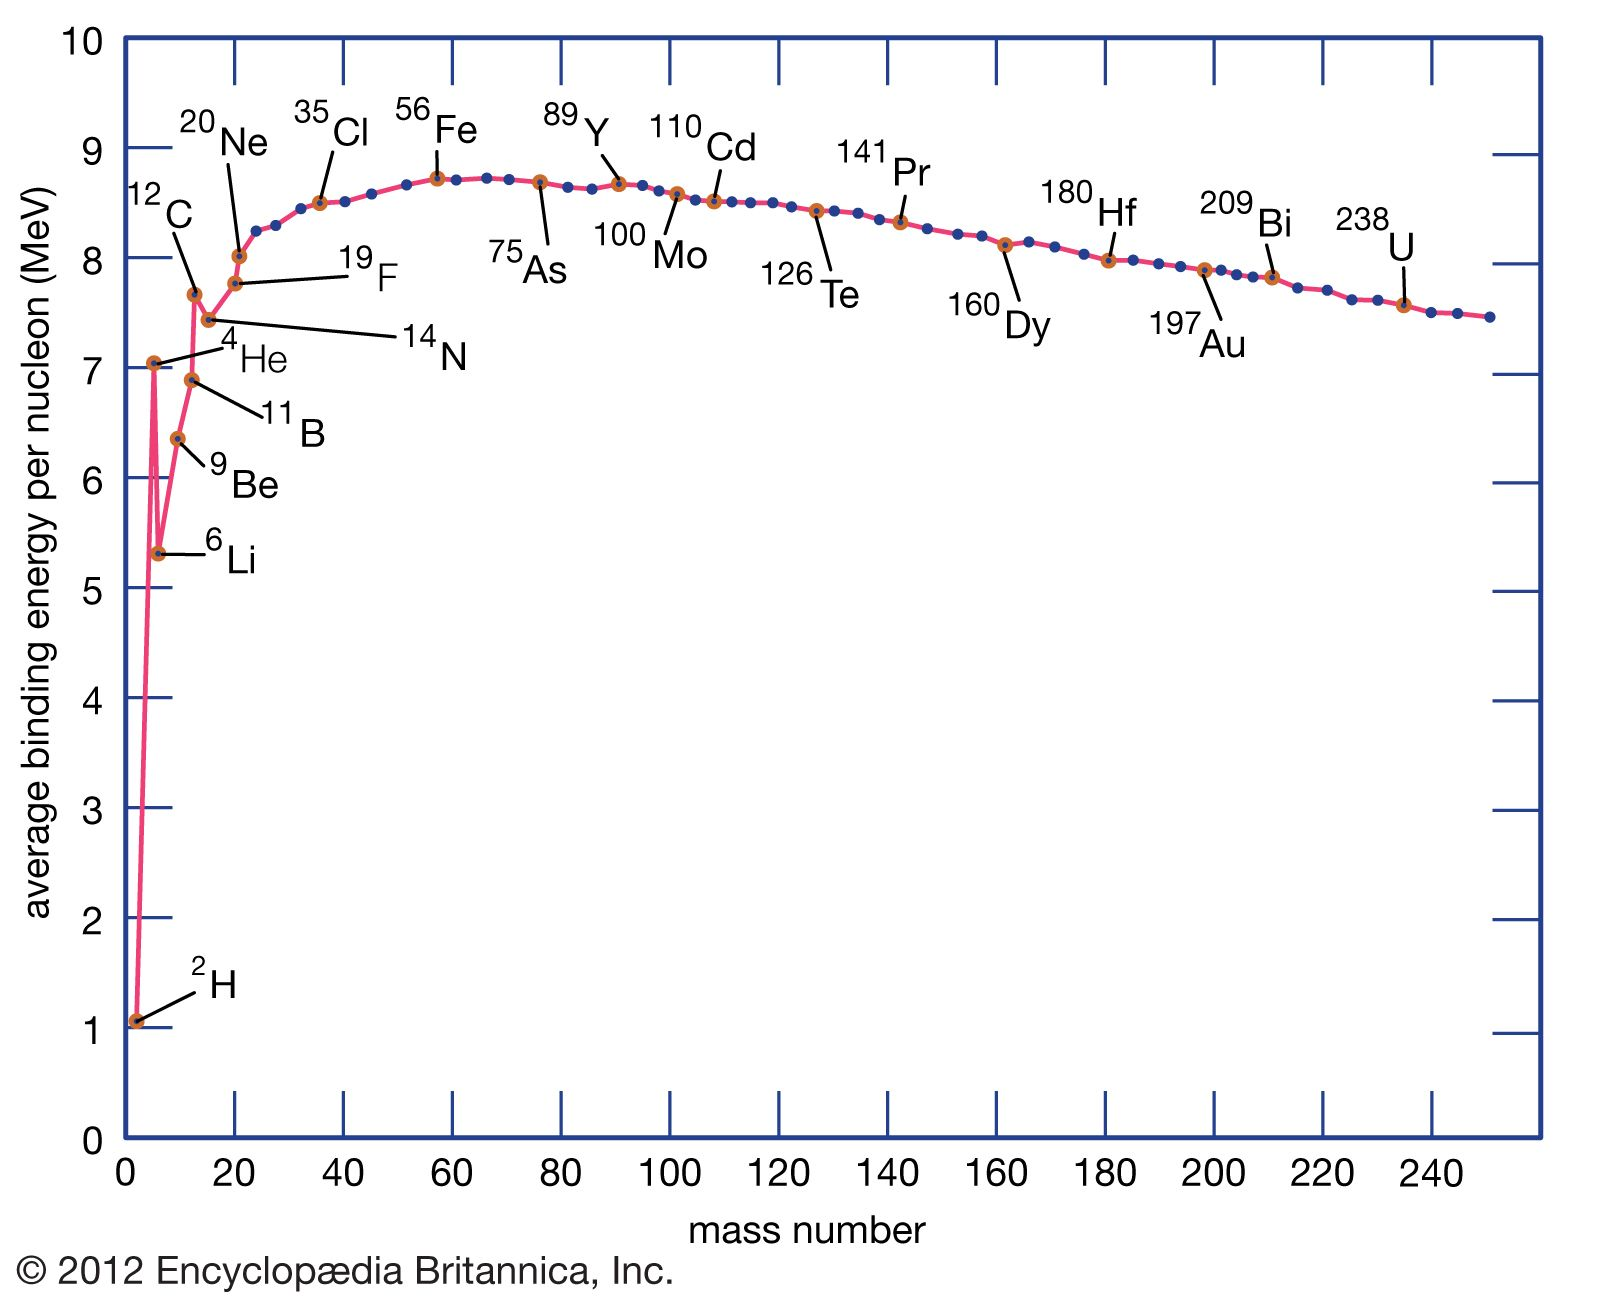
\includegraphics[width=0.6\linewidth]{graphics/energies-function-atomic-mass-number-2241843032.jpg}
            \caption{Binding energy per nucleon as a function of mass number $A$. The curve rises to a maximum near iron and nickel, and falls off slowly for heavier nuclei.}
            \label{fig:binding-energy-curve}
        \end{figure}

        Plotted against $A$ it gives the binding-energy curve, and almost all of nuclear energetics is contained in its shape. It rises steeply through the light nuclei, reaches a broad maximum of about \qty{8.8}{\mega\electronvolt} per nucleon near $A \simeq 56$--$62$ (iron and nickel), and then falls slowly, to about \qty{7.6}{\mega\electronvolt} for uranium. A reaction releases energy whenever it moves nucleons to a higher point on this curve. Which way that is depends entirely on where you start, so neither mechanism is a source of energy in itself---fusing nuclei heavier than iron costs energy, and so does splitting nuclei lighter than it.

        Light nuclei therefore climb by \emph{fusing} together and heavy nuclei by \emph{splitting} apart, both running towards iron from their respective sides. Fusing hydrogen into helium releases about \qty{7}{\mega\electronvolt} per nucleon. Uranium sits only about \qty{0.9}{\mega\electronvolt} per nucleon below the peak, so splitting one $235$-nucleon nucleus releases roughly $235 \times 0.9 \simeq \qty{200}{\mega\electronvolt}$---an enormous figure per event, simply because so many nucleons move at once, but some eight times less per nucleon than fusion delivers.

        The curve itself is reproduced by the \emph{semi-empirical mass formula} of the liquid-drop model: a volume term proportional to $A$, a surface term penalising small nuclei, a Coulomb term penalising large $Z$, an asymmetry term favouring $N \simeq Z$, and a pairing term. The pairing term is what puts the local jumps into an otherwise smooth curve, since nuclei with even $Z$ and even $N$ are more tightly bound than their odd neighbours.

    \subsection{Structure and reactions}

        Two models capture the structure. The \emph{liquid-drop model} treats the nucleus like a drop of incompressible fluid, with the strong force and the electrostatic repulsion playing the roles of surface tension and internal pressure. It reproduces the gross trend of the binding energy and explains why very heavy nuclei can split. The \emph{shell model}, by analogy with atomic electron shells (\cref{sec:atom-molecule}), has nucleons filling discrete energy shells. It explains the deviations from the liquid-drop trend and the \emph{magic numbers} $2, 8, 20, 28, 50, 82, 126$, at which nuclei are especially tightly bound.

        Nuclear reactions transform nuclei, often under bombardment by neutrons or protons:

        \begin{itemize}
            \item \textbf{fission} --- a heavy nucleus splits into two (or more) lighter ones, releasing neutrons and a large amount of energy. The released neutrons can trigger further fissions, which is the chain reaction. A typical case is ${}^{235}\mathrm{U} + n \rightarrow {}^{141}\mathrm{Ba} + {}^{92}\mathrm{Kr} + 3n$.
            \item \textbf{fusion} --- two light nuclei merge into a heavier one, releasing energy, but only if they can be brought within range of the strong force against their electrostatic repulsion (\cref{sec:nucleosynthesis}). The easiest reaction to drive is ${}^{2}\mathrm{H} + {}^{3}\mathrm{H} \rightarrow {}^{4}\mathrm{He} + n$, worth \qty{17.6}{\mega\electronvolt}.
            \item \textbf{alpha decay} --- emission of an alpha particle (a helium-4 nucleus), which is itself a tunnelling process (\cref{sec:tunnelling}), as in ${}^{238}\mathrm{U} \rightarrow {}^{234}\mathrm{Th} + \alpha$.
            \item \textbf{beta decay} --- emission of an electron ($\beta^{-}$, a neutron turning into a proton, with an electron \emph{antineutrino}) or of a positron ($\beta^{+}$, the reverse, with a neutrino), via the weak interaction. Examples are ${}^{14}\mathrm{C} \rightarrow {}^{14}\mathrm{N} + e^{-} + \bar{\nu}_{e}$ and ${}^{22}\mathrm{Na} \rightarrow {}^{22}\mathrm{Ne} + e^{+} + \nu_{e}$. What happens underneath, one quark changing flavour, is in \cref{sec:interactions}.
            \item \textbf{electron capture} --- the nucleus absorbs one of its own innermost atomic electrons, which converts a proton into a neutron and emits a neutrino, as in ${}^{40}\mathrm{K} + e^{-} \rightarrow {}^{40}\mathrm{Ar} + \nu_{e}$. It competes with $\beta^{+}$ decay, has the same effect on $Z$ and $N$, and is the only route open when there is too little energy available to create a positron.
            \item \textbf{gamma decay} --- emission of a high-energy photon by an excited nucleus returning to its ground state, usually following one of the above. It changes neither $Z$ nor $N$, only the energy: ${}^{60}\mathrm{Co}$ beta-decays to an excited ${}^{60}\mathrm{Ni}$, which then sheds two gamma photons.
        \end{itemize}

        Both directions have been engineered. A reactor runs a controlled chain reaction in ${}^{235}$U or ${}^{239}$Pu, with a moderator to slow the neutrons and control rods to absorb the surplus, while a fission bomb is the same chain reaction left uncontrolled in a supercritical mass. Controlled fusion is not yet a power source, the large experiments being ITER and the National Ignition Facility, whereas a thermonuclear bomb solves the confinement problem crudely by using a fission stage to ignite the fusion fuel.

        A \emph{decay chain}, also called a radioactive decay series, is a succession of decays leading from one unstable nuclide to the next until a stable one is reached. There are four such chains in principle, but only three occur naturally today: the thorium, uranium and actinium series. The fourth, the neptunium series, has died out. Its longest-lived member, ${}^{237}$Np, has a half-life of about $2.1$ million years, so in the $4.5$ billion years since the Earth formed roughly two thousand half-lives have passed and nothing of the original stock survives.

    \subsection{Borders of stability of nuclides}

        Add protons or neutrons to a nucleus indefinitely and at some point it will not hold them: the next one is simply not bound, and falls straight back out. The lines on the chart of nuclides where that happens are the \emph{drip lines}, one for protons and one for neutrons, and they mark the edges of the world of nuclides. For the heaviest nuclei a third limit intervenes before either drip line is reached, namely spontaneous fission.

        \begin{itemize}
            \item \textbf{The proton drip line} --- protons are held in by the Coulomb barrier even once they are formally unbound, which lengthens the lifetimes near the edge and makes that edge comparatively easy to reach. It is mapped, firmly or tentatively, up to about $Z=84$, and proton-rich nuclides have been made as far as neptunium ($Z=93$).
            \item \textbf{The neutron drip line} --- neutrons feel no Coulomb barrier, so nothing holds them in and the neutron-rich edge is far harder to reach. It is established experimentally only up to neon ($Z=10$), and pushing it further is a major current effort.
            \item \textbf{Superheavy nuclei} --- here the nucleus splits before it runs out of room for nucleons, so the limit is spontaneous fission rather than binding. What stability these nuclei have comes from shell effects, and whether there is a genuine \enquote{island of stability} of long-lived superheavy nuclides remains open.
        \end{itemize}

\section{Nucleosynthesis and sources of energy of stars}
\label{sec:nucleosynthesis}\todoans{Yes, it is the umbrella term: any process that builds atomic nuclei out of pre-existing nucleons or lighter nuclei, which is precisely the four routes listed below. What it does \emph{not} cover is the making of the nucleons themselves out of quarks in the first microsecond---that goes under baryogenesis and hadronisation, and is a stage earlier than anything called nucleosynthesis.}

    Elements are produced in four natural ways: \emph{primordial nucleosynthesis} just after the Big Bang, \emph{fusion inside stars}, \emph{neutron capture} in and around dying stars, and \emph{spallation} by cosmic rays.

    \paragraph{The Big Bang: $Z \leq 4$}

    The first protons formed once the Universe had cooled enough for quarks to bind into hadrons (roughly \qtyrange{1e-6}{1}{\second} after the Big Bang). \emph{Primordial nucleosynthesis} then followed (about \qtyrange{10}{1e3}{\second}), producing the light nuclei: deuterium ($^{2}$H), tritium ($^{3}$H), helium ($^{3}$He and $^{4}$He), lithium ($^{7}$Li) and beryllium ($^{7}$Be). It stopped there because \emph{no stable nuclide has $A = 5$ or $A = 8$,} so there is no way to build upwards by adding one nucleon at a time, and the Universe thinned and cooled too fast for anything slower.

    \paragraph{Stars: $Z$ up to $26$}

    \emph{Stars} formed much later and drove the next round. They \emph{fuse hydrogen into helium, then helium into carbon} (three $^{4}$He nuclei at once, the triple-alpha process, which is how the $A=8$ gap is bridged), and in the more massive stars carbon, neon, oxygen and silicon \emph{burn} in turn---burning here meaning the fusion of a given fuel, with nothing chemical about it---each stage requiring a higher temperature than the last and building nuclei up to iron. There it stops. It is often said that fusion \enquote{stops at iron} because $^{56}$Fe is the most stable nucleus, but this needs care: $^{56}$Fe has the smallest \emph{mass per nucleon}, whereas the largest \emph{binding energy per nucleon} belongs to nickel, $^{62}$Ni (the two differ because the proton and neutron masses are not equal). In practice stellar fusion favours $^{56}$Ni, which is less stable and decays to $^{56}$Fe. Either way, past the peak of the binding-energy curve (\cref{sec:nuclei}) \emph{fusion would consume energy rather than release it}, so it can no longer support the star.

    \paragraph{Neutron capture: $Z$ above $26$}

    Everything heavier is built not by fusion but by adding neutrons, which feel no Coulomb repulsion and so need no barrier to be overcome, followed by $\beta^{-}$ decay of the neutron-rich product (\cref{sec:nuclei}). Two regimes are distinguished by how the capture rate compares with the decay rate. The \emph{s-process} (slow) proceeds in the interiors of evolved low-mass stars, one neutron at a time with leisure to decay in between, and it builds the nuclides lying along the valley of stability up to bismuth. The \emph{r-process} (rapid) dumps many neutrons on a nucleus before any decay can occur, requires an extreme neutron flux, and is responsible for the most neutron-rich heavy nuclides, gold, platinum, thorium and uranium among them. Supernovae were long assumed to be its site, and the merger of two neutron stars observed in $2017$ confirmed at least one such site directly.

    \paragraph{Cosmic rays: lithium, beryllium and boron}

    \emph{Cosmic rays} are high-energy charged particles---about nine parts in ten protons, most of the remainder helium nuclei---and not electromagnetic radiation at all, despite the name and despite any confusion with the cosmic microwave background, which is a separate thing entirely. Most of them are flung out by supernova remnants within our own galaxy, the gentlest come from the Sun, and the very highest energies come from outside the galaxy altogether.

    These three light elements are an exception on both counts: stars destroy them rather than make them, and the Big Bang made only a trace of lithium. They come instead from \emph{spallation}, in which a fast cosmic-ray proton strikes a heavier nucleus in the interstellar medium and chips fragments off it.

    \subsection{Thermonuclear fusion}

        A \emph{thermonuclear reaction} is fusion driven by heat: the nuclei get the kinetic energy they need to reach one another from the thermal motion of a hot plasma, so the \enquote{thermo} describes how the barrier is beaten rather than what comes out.\todoans{The same nuclear process as fusion (\cref{sec:nuclei}), so every thermonuclear reaction is fusion but not every fusion is thermonuclear. The word fixes only the input side---nuclei brought together by thermal motion, as in a stellar core or a hydrogen bomb. Fusion can also be driven cold, by firing a beam at a fixed target in an accelerator, or by muon catalysis, where a muon takes the electron's place and shrinks the molecule until the two nuclei touch. The products are the same either way, kinetic energy of the fragments plus gamma rays.} Being exothermic, it releases energy---as kinetic energy of the products and as gamma rays---which is then shared with the surroundings as heat. The energy released can be found from the mass defect (\cref{eq:mass-defect}).

        For hydrogen nuclei (protons) to fuse they must come within the range of the strong force (about \qty{1}{\femto\metre}), but they first have to overcome their mutual electrostatic repulsion, a barrier of order \qty{1}{\mega\electronvolt}. Classically this needs a temperature of about \qty{1e10}{\kelvin}, far hotter than any stellar core. Fusion nonetheless proceeds at the much lower core temperatures because of \emph{quantum tunnelling} (\cref{sec:tunnelling}), which lets protons pass through the barrier rather than over it.

    \subsection{The proton--proton chain (the Sun)}

        The \emph{proton--proton chain} is the sequence of reactions that builds one helium nucleus from four protons, releasing energy at each step. It answers both halves of the question at once: it is the main energy source of the Sun and of similar stars, and, since it makes helium out of hydrogen, it is nucleosynthesis as well. It operates in stellar cores at temperatures of a few to a few tens of millions of kelvin. In its commonest branch:

        \begin{keyeq}{eq:pp-chain}{Proton--proton chain}
            \begin{aligned}
            p + p           &\rightarrow {}^{2}\mathrm{H} + e^{+} + \nu_{e} \\
            {}^{2}\mathrm{H} + p &\rightarrow {}^{3}\mathrm{He} + \gamma \\
            {}^{3}\mathrm{He} + {}^{3}\mathrm{He} &\rightarrow {}^{4}\mathrm{He} + 2p  ,
            \end{aligned}
        \end{keyeq}

        which overall converts four protons into one $^{4}$He nucleus, two positrons and two neutrinos, releasing about \qty{26.7}{\mega\electronvolt}. The first step is the bottleneck, and it is what makes the Sun burn slowly enough to have a long life: it requires one of the two protons to turn into a neutron by the weak interaction (\cref{sec:interactions}) at the very moment of contact, which is an exceedingly improbable coincidence. The neutrinos escape immediately and are the only direct evidence we have of the core, while the photons take a very long time to random-walk their way out. In stars appreciably more massive than the Sun, and hence hotter, the \emph{CNO cycle} takes over instead, using carbon, nitrogen and oxygen as catalysts to achieve the same net conversion.

\section{Classification of elementary particles; quarks, leptons and force carriers, structure of hadrons}
\label{sec:particles}

    A particle is \emph{elementary} if it has no known internal structure: nothing smaller has ever been found inside it, and the theory treats it as a point. Quarks, leptons, the force carriers and the Higgs boson are elementary on present evidence, whereas a proton is not, being made of quarks. The full inventory is \cref{fig:standard-model}, and what these particles do to one another---carriers, ranges, strengths---is \cref{sec:interactions}.

    \begin{figure}[H]
        \centering
        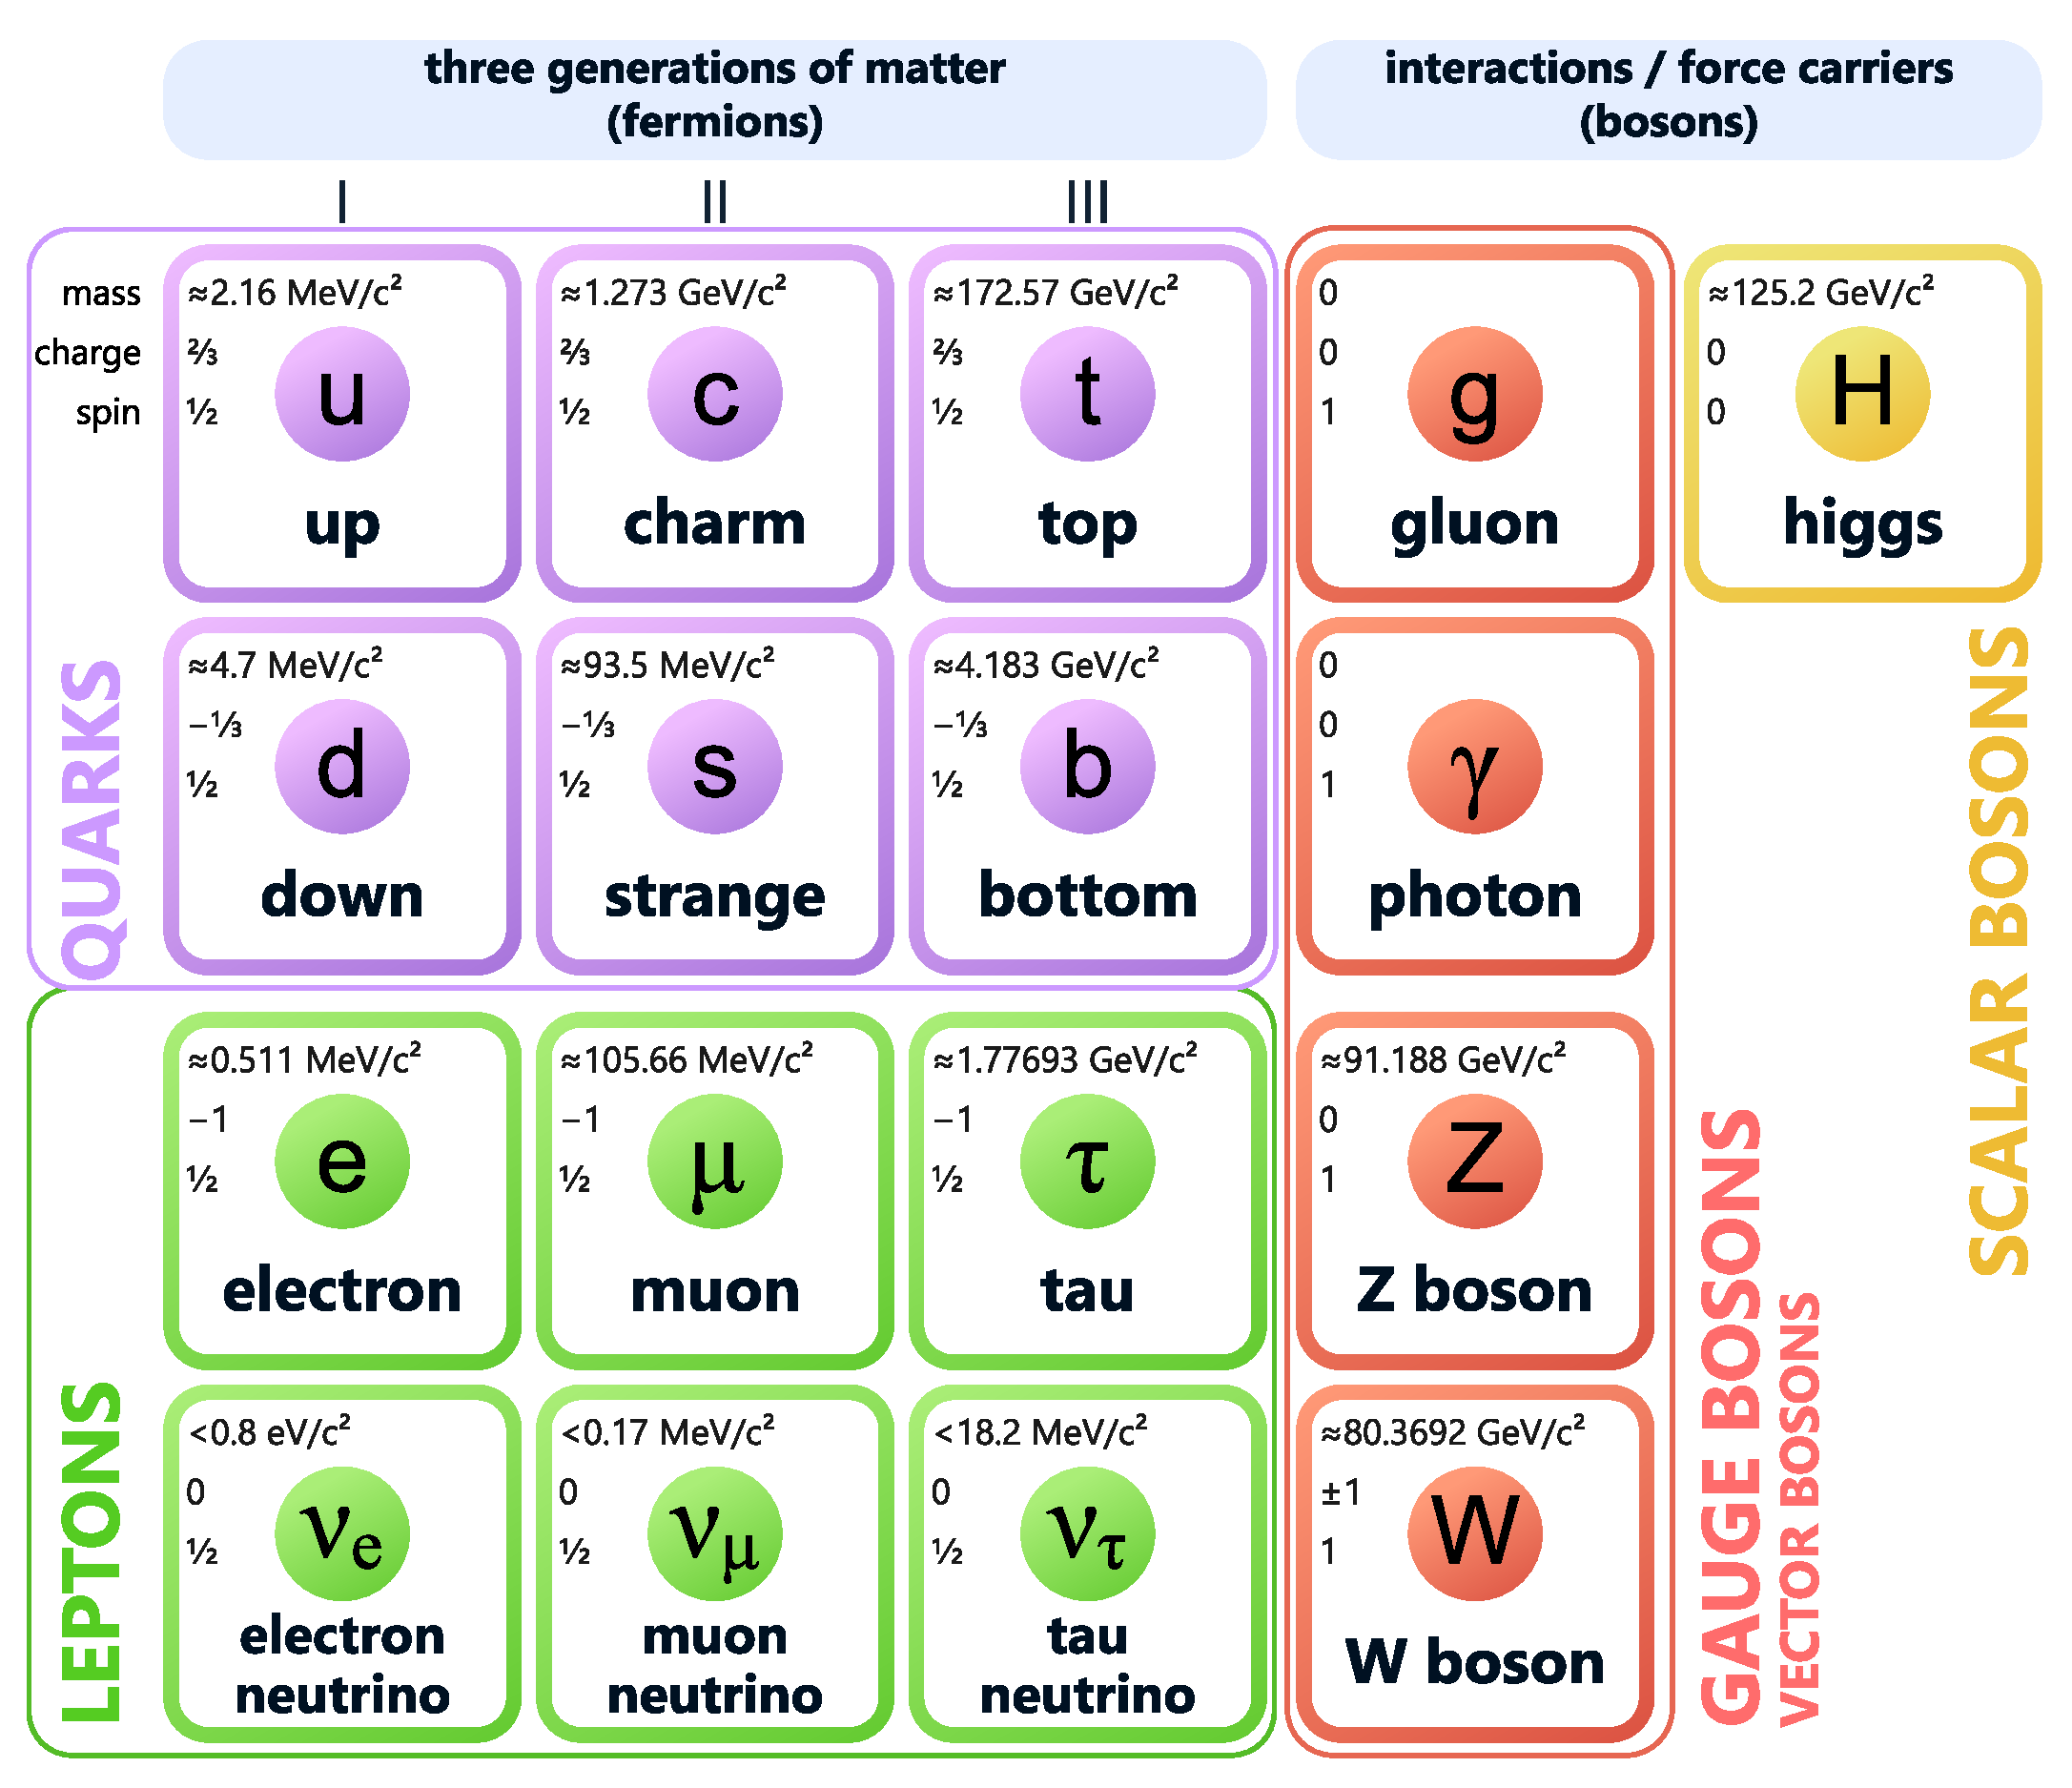
\includegraphics[width=0.68\linewidth]{graphics/Standard_Model_of_Elementary_Particles.pdf}
        \caption{The Standard Model: three generations of quarks and leptons, the force carriers, and the Higgs boson.}
        \label{fig:standard-model}
    \end{figure}

    Two cuts run through the classification, and they are independent of one another:

    \begin{itemize}
        \item \textbf{fermion or boson} --- a \emph{fermion} has half-integer spin and obeys the Pauli exclusion principle, so no two may share a state, whereas a \emph{boson} has integer spin and any number may share one (\cref{sec:indistinguishability}). Matter is made of fermions, forces are carried by bosons.
        \item \textbf{elementary or composite} --- \emph{quarks} and \emph{leptons} are the elementary fermions, while a \emph{hadron} is a composite particle built out of quarks and held together by the strong interaction.
    \end{itemize}

    \subsection{Quarks and leptons}

        A \emph{lepton} is an elementary fermion that does not feel the strong interaction and can therefore exist on its own. The six come in three pairs, plus their antiparticles:

        \begin{itemize}
            \item the electron and the electron neutrino,
            \item the muon and the muon neutrino,
            \item the tau and the tau neutrino.
        \end{itemize}

        The three charged leptons carry electric charge $-1$ (their antiparticles $+1$), while the three neutrinos are electrically neutral. All of them feel the weak interaction.

        A \emph{quark} is an elementary fermion that does feel the strong interaction, because it carries \emph{colour charge} (\cref{sec:interactions}), and is never found on its own. The six \enquote{flavours}, plus antiquarks, are:

        \begin{itemize}
            \item up (u), charge $+\nicefrac{2}{3}$,
            \item down (d), charge $-\nicefrac{1}{3}$,
            \item strange (s), charge $-\nicefrac{1}{3}$,
            \item charm (c), charge $+\nicefrac{2}{3}$,
            \item bottom (b), charge $-\nicefrac{1}{3}$,
            \item top (t), charge $+\nicefrac{2}{3}$.
        \end{itemize}

        Both sets are grouped into three \emph{generations}---up and down, charm and strange, top and bottom for the quarks, with the three lepton pairs above in the same order---each generation a heavier copy of the one before. Ordinary matter uses only the first, up and down quarks and the electron, since everything in the other two decays within a fraction of a second.

    \subsection{Force carriers}

        The interactions are carried by spin-1 bosons: eight massless \emph{gluons} for the strong interaction, the massless \emph{photon} for the electromagnetic one, and the heavy $W^{+}$, $W^{-}$ and $Z^{0}$ for the weak. Gluons themselves carry colour, which is why they attract one another and why the strong interaction behaves unlike the other three. The spin-0 \emph{Higgs boson} is not a force carrier at all but the quantum of the field that gives the $W$, the $Z$ and the charged fermions their masses. Carrier masses, ranges and relative strengths are collected in \cref{tab:interactions}.

    \subsection{The structure of hadrons}

        A hadron must be \emph{colour-neutral} overall, and there are exactly two ways of arranging that. Three quarks, one of each colour, make a \emph{baryon}, the proton ($uud$, \cref{fig:proton}) and the neutron ($udd$) being the two that matter. A quark together with an antiquark of the matching anticolour makes a \emph{meson}, the lightest being the pion. Baryons are therefore composite fermions and mesons composite bosons, which is the two cuts above crossing each other.

        Electric charge is simply the sum of the quark charges: $+\nicefrac{2}{3}+\nicefrac{2}{3}-\nicefrac{1}{3}=+1$ for the proton and $+\nicefrac{2}{3}-\nicefrac{1}{3}-\nicefrac{1}{3}=0$ for the neutron. Mass is not additive in the same way---almost all of a hadron's mass is the energy of the gluon field binding the quarks rather than the quark masses themselves (\cref{sec:interactions}). A useful bookkeeping quantum number is the \emph{baryon number}, $+1$ for a baryon, $-1$ for an antibaryon and $0$ for a meson, conserved in every interaction so far observed, which is why the proton, being the lightest baryon, has nothing it could decay into.

        Baryons are what ordinary matter is made of, but ordinary matter is a small part of the whole: baryonic matter is about $5\%$ of the energy content of the Universe, non-baryonic \emph{dark matter} about $27\%$ and \emph{dark energy} the remaining $68\%$, so of everything that gravitates, some five parts in six are dark. The two dark components are not variants of one thing---dark matter is matter, which clumps and attracts and is what holds galaxies together, whereas dark energy is a property of empty space itself, spread perfectly evenly and pushing, and is what makes the expansion of the Universe accelerate. Neither is odd in its mass: dark matter has ordinary mass and gravitates normally, and what is dark about it is only that it neither emits nor absorbs light. \emph{Antimatter} likewise has ordinary positive mass and falls downwards like anything else---there is no negative mass---and the open question about it is why so little of it survived, when the Big Bang should have made equal amounts.

\section{Band structure of electron states in crystals; metals, semiconductors, insulators}
\label{sec:bands}

    Band theory is the quantum-mechanical account of electrical conduction. Unlike the classical picture, it starts from the wave nature of electrons and from \emph{Fermi--Dirac} statistics (\cref{eq:fermi-dirac}). Its central idea is the \emph{energy band}: a continuous range of energies that electrons in a solid may occupy.

    The bands arise in the same way as molecular orbitals do (\cref{sec:atom-molecule}), only carried to the limit. Bring two atoms together and each atomic level splits in two, and in general $N$ atoms give $N$ levels, because once the orbitals overlap the Pauli exclusion principle (\cref{sec:indistinguishability}) will not let the electrons all remain in one and the same state.\todoans{As many levels as there are atoms, not always two---two atoms merely happen to give two. The mechanism is orbital overlap. Far apart, the atoms' orbitals are independent and their levels coincide. As they approach, the two orbitals can combine either in phase or out of phase: the in-phase (bonding) combination piles electron density between the nuclei and lies lower in energy, the out-of-phase (antibonding) one has a node between them and lies higher. Pauli is what forces the split to happen at all, and its size grows with the overlap, which is why the outer bands are wide while the inner levels are barely split.} Bring $10^{23}$ together in a crystal and each level splits into $10^{23}$ levels so closely spaced as to form a continuous band.

    Between the bands lie \emph{forbidden gaps} in which no electron state exists at all, and these are a consequence of the periodicity of the lattice. An electron wave whose wavelength fits the lattice spacing satisfies the Bragg condition (\cref{eq:bragg}) and is reflected straight back on itself, so the forward and backward waves add to a standing wave, which carries nothing anywhere. At those energies there is simply no travelling state for an electron to occupy, and that absence is the gap.

    For the outer (valence) electrons two bands matter:

    \begin{itemize}
        \item the \textbf{valence band} --- the energies of electrons still bound to their atoms,
        \item the \textbf{conduction band} --- the energies of electrons freed from their atoms, which can then carry current.
    \end{itemize}

    Whether a solid conducts depends not on how many electrons it has but on whether a band is partly empty. In a completely full band every state is occupied, so an applied field has nowhere to move an electron to: for every electron it would accelerate one way there is another going the other way, and the two cancel exactly. Only a partly filled band leaves states free just above the occupied ones, and only then can a field produce a net drift. The energy dividing occupied from empty states is the \emph{Fermi level} (\cref{subsec:quantum-statistics}), and what matters is whether it falls inside a band or inside a gap. It does shift with temperature, negligibly so in a metal, but appreciably in a semiconductor, where it lies near the middle of the gap and moves with both temperature and doping.

    The size of the gap sorts materials into three classes:

    \begin{itemize}
        \item \textbf{Metals} have no gap: either the valence band is only partly filled, so its electrons move freely, or the valence and conduction bands overlap. Either way the Fermi level lies within a band, there are many mobile electrons and current flows easily.
        \item \textbf{Semiconductors} have a small gap (for example Ge $\simeq\qty{0.7}{\electronvolt}$, Si $\simeq\qty{1.1}{\electronvolt}$, GaAs $\simeq\qty{1.4}{\electronvolt}$). At absolute zero the conduction band is empty and the material is an insulator, but at higher temperatures electrons are thermally excited across the gap, leaving mobile \enquote{holes} behind in the valence band---a hole being the vacancy a departed electron leaves, which drifts and conducts as though it were a positive charge (\cref{tab:conduction-kinds})---so that conductivity rises with temperature, the opposite of a metal (\cref{sec:electric-field}). Semiconductors can also be \emph{doped}: adding donor atoms with one valence electron too many gives an n-type semiconductor, adding acceptor atoms with one too few gives a p-type one. Joining the two makes a p--n junction, which passes current in one direction only, and that junction is the basis of the diode, the transistor and the solar cell.
        \item \textbf{Insulators} have a large gap, conventionally above about \qtyrange{3}{4}{\electronvolt} (diamond has \qty{5.5}{\electronvolt}), so almost no electrons reach the conduction band and current barely flows.
    \end{itemize}

    The same gap also decides what the material looks like. Visible light spans \qtyrange{380}{750}{\nano\metre} (\cref{sec:spectroscopy}), which in photon energy is roughly \qtyrange{1.7}{3.3}{\electronvolt}. A semiconductor whose gap is around \qty{1}{\electronvolt} therefore has a state waiting for every visible photon, absorbs the lot and looks opaque, whereas an insulator whose gap exceeds \qty{3.3}{\electronvolt} offers a visible photon nowhere to put an electron and is transparent. That is why diamond and quartz are clear and silicon is not.